%%%%%%%%%%%%%%% Page Setup %%%%%%%%%%%%%%%

\documentclass[a4paper, 11pt]{book}
\usepackage[utf8]{inputenc}
\usepackage[framemethod=tikz]{mdframed}
\usepackage[margin=3cm]{geometry}
\setlength\parindent{0pt}
\setlength{\parskip}{\baselineskip}%
\usepackage{graphicx}
\usepackage{tgadventor}
%\renewcommand*\familydefault{\sfdefault}
\usepackage[T1]{fontenc}
\usepackage{bm}

%%%%%%%%%%%%%%% Math Stuff %%%%%%%%%%%%%%%

\usepackage{amsmath}
\usepackage{amssymb}
\usepackage{tikz}
\usepackage{tikz-cd}
\usepackage{tkz-euclide}
\usepackage{pgf-pie}
\usepackage{cancel}

%%%%%%%%%%%%%%% Quotation Stuff %%%%%%%%%%%%%%%

\usepackage[english]{babel}
\usepackage[autostyle]{csquotes}

%%%%%%%%%%%%%%% Color %%%%%%%%%%%%%%%

\definecolor{p}{rgb}{0.9118, 0.4961, 0.6804}
\definecolor{p1}{rgb}{1, 0.92, 0.963}
\definecolor{g}{rgb}{0.023, 0.477, 0.219}
\definecolor{g1}{rgb}{0.03, 0.75, 0.20}
\definecolor{g2}{rgb}{0.95, 1, 0.95}

%%%%%%%%%%%%%%% Link Setup %%%%%%%%%%%%%%%

\usepackage{hyperref}
\hypersetup{colorlinks=true, linkcolor=g, filecolor=g, urlcolor=g,}

%%%%%%%%%%%%%%% Box %%%%%%%%%%%%%%%

\newmdenv[innerlinewidth=2pt, roundcorner=4pt,linecolor=g1,innerleftmargin=20pt,
innerrightmargin=20pt,innertopmargin=20pt,innerbottommargin=20pt,backgroundcolor = g2]{mybox}

%%%%%%%%%%%%%%% Border Stuff %%%%%%%%%%%%%%%

\usepackage{fancyhdr}
\pagestyle{fancy}
\fancyhf{}
\fancyhead[LE,RO]{\leftmark}
\fancyhead[RE,LO]{\thepage}
\fancyfoot[CE,CO]{}
\fancyfoot[LE,RO]{}

%%%%%%%%%%%%%%% Bug Fix Adjustments %%%%%%%%%%%%%%%

\setlength{\headheight}{14pt}
\setlength{\footskip}{55pt}

%%%%%%%%%%%%%%% Index %%%%%%%%%%%%%%%

\usepackage{makeidx}
\makeindex

%%%%%%%%%%%%%%% Custom Commands %%%%%%%%%%%%%%%

\def\greenlozenge{\mathbin{\color{g}\blacklozenge}}

\newcommand{\emphasis}[1]{\underline{\textbf{#1}} }
\newcommand{\vocab}[1]{\underline{\textbf{#1}}\index{#1}}

\newcommand{\claim}{\textbf{\underline{Claim}} }
%\newcommand{\corollary}{\underline{\textbf{Corollary}} }
\newcommand{\defn}{\underline{\textbf{Def}} }
\newcommand{\digression}{\underline{\textbf{Digression}} }
\newcommand{\easy}{\underline{\textbf{Easy}} }
\newcommand{\example}{\underline{\textbf{Example}} }
\newcommand{\fact}{\underline{\textbf{Fact}} }
\newcommand{\facts}{\underline{\textbf{Facts}} }
\newcommand{\goal}{\underline{\textbf{Goal}} }
\newcommand{\idea}{\underline{\textbf{Idea}} }
%\newcommand{\lemma}{\underline{\textbf{Lemma}} }
\newcommand{\need}{\underline{\textbf{Need}} }
\newcommand{\note}{\underline{\textbf{Note}} }
\newcommand{\proof}{\underline{\textbf{Proof}} }
\newcommand{\recall}{\underline{\textbf{Recall}} }
\newcommand{\remark}{\underline{\textbf{Remark}} }
%\newcommand{\theorem}{\underline{\textbf{Theorem}} }
\newcommand{\verify}{\underline{\textbf{Verify}} }


%%%%%%%%%%%%%%% New Theorems %%%%%%%%%%%%%%%


\newtheorem{theorem}{Theorem}[section]
\newtheorem{corollary}{Corollary}[theorem]
\newtheorem{lemma}[theorem]{Lemma}
\newtheorem{conjecture}[theorem]{Conjecture}

%%%%%%%%%%%%%%% Math Operators %%%%%%%%%%%%%%%
\DeclareMathOperator{\A}{\mathbb{A}}
\DeclareMathOperator{\Aut}{Aut}
\DeclareMathOperator{\C}{\mathbb{C}}
\DeclareMathOperator{\characteristic}{char}
\DeclareMathOperator{\cod}{cod}
\DeclareMathOperator{\dom}{dom}
\DeclareMathOperator{\Fix}{Fix}
\DeclareMathOperator{\Frac}{Frac}
\DeclareMathOperator{\Free}{Free}
\DeclareMathOperator{\id}{id}
\DeclareMathOperator{\Ima}{Im}
\DeclareMathOperator{\Mor}{Mor}
\DeclareMathOperator{\N}{\mathbb{N}}
\DeclareMathOperator{\Obj}{Obj}
\DeclareMathOperator{\Q}{\mathbb{Q}}
\DeclareMathOperator{\R}{\mathbb{R}}
\DeclareMathOperator{\Res}{Res}
\DeclareMathOperator{\Stab}{Stab}
\DeclareMathOperator{\Span}{span}
\DeclareMathOperator{\Spec}{Spec}
\DeclareMathOperator{\trdeg}{trdeg}
\DeclareMathOperator{\Z}{\mathbb{Z}}
%%%%%%%%%%%%%%% Title %%%%%%%%%%%%%%%

\title{Transcendental Numbers}
\author{Vincent Lin}
\date{December 15, 2023}
\begin{document}
\frontmatter
\maketitle
\tableofcontents
\chapter{Preface}
\indent Starting from the background information from 21441 and algebra, we will discuss transcendental numbers. Then, we will introduce methods of explicitly constructing, finding, and detecting transcendental numbers. We will talk about some additional algebra preliminaries and theorems from complex analysis. We will name several classes of transcendental numbers, and the specific methods of finding them will be discussed. The main theorems include the Lindemann-Weierstrass theorem, Gelfond-Schneider theorem, and Baker's theorem. Then, we conclude with a discussion of Schanuel's conjecture and its consequences. The main sequence of theorems is primarily related to determining the transcendence of complex numbers using auxiliary functions.
\mainmatter{}
\chapter{Preliminaries}
\section{Algebraic and Transcendental Numbers}
\subsection{Definitions and Motivation}
\defn{An \vocab{algebraic number} is $\alpha \in \C$ which is the root of a nonzero polynomial in $\Q[x]$ (equivalently the root of a nonzero polynomial in $\Z[x]$). A \vocab{transcendental number} is a complex number that is not algebraic.}\par

\note{We will use $\A$ to denote the set of algebraic numbers and we will use $\C \setminus \A$ to denote the set transcendental numbers. We will use $\R \setminus \A$ to denote the set of real transcendental numbers.}\par

To find examples of algebraic numbers, we can take any nonzero polynomial in $\Q[x]$ find its roots. By definition, these roots are algebraic numbers. For example, $\sqrt{2}$ is algebraic because it is a root of $x^2 - 2$. Also, $i$ is algebraic because it is the root of $x^2 + 1$. All rational numbers are algebraic as well. Let $\frac{p}{q} \in \Q$ be rational, where $p, q \in \Z$ and $q$ is nonzero. Then, it is the root of $x - \frac{p}{q}$. Therefore, $\Q \subseteq \A$.\par

What about transcendental numbers? Do they exist?\par

\begin{mybox}
    \theorem{Yes, transcendental numbers exist.}
\end{mybox}

\proof{Consider the set of algebraic numbers, which we will denote by $\A$. This set is countable. We will show this by forming a surjection  \[\phi : \left(\N \times \bigcup\limits_{n \in \N} \Q^{n}\right) \to \A.\] Note that $\N \times \bigcup\limits_{n \in \N} {\Q}^{n}$ is countable because it is the Cartesian product of a countable set with a countable union of countable sets. By the fundamental theorem of algebra, we know that a polynomial of degree $k$ has $k$ (not necessarily distinct) roots. Therefore, we can number the $k$ roots from $1$ to $k$ for each polynomial. Thus, if we specify the nonzero rational coefficients $(a_0, \ldots, a_k)$ and an index $i$ for $i \in [k]$ to be the $i$-th root of the polynomial $a_k x^k + \cdots + a_0$, we get an algebraic number. We define the map $\phi(i, (a_0, \ldots, a_k))$ to be the $i$-th root of $a_k x^k + \cdots + a_0$ if it exists. Otherwise, we map the input to zero. From the definition, we know that every algebraic number can be encoded this way since it is one of the roots of a nonzero rational polynomial. Thus, for all $a \in \A$, there must be an input $x$ such that $\phi(x) = a$, making this a surjective map from a countable set to $\A$. This makes $\A$ countable. However, since $\C$ is uncountable, it cannot be the case that all complex numbers are algebraic. Thus, if a complex number is not algebraic, it must be transcendental. Furthermore, $\R$ is uncountable so there must be real transcendental numbers as well.\[ \greenlozenge \]}

If transcendental numbers exist, then can we find an example? To show that a number is algebraic, we have to find a nonzero rational polynomial that it is a root of, evaluate that polynomial at that number, and verify that we get zero. However, checking if a number is transcendental is a very hard problem. The rest of this paper will discuss the transcendence of a large class of numbers and methods for determining transcendence.\par

\subsection{Diagonalization}
Luckily, uncountability tells us a lot of information about transcendental numbers already. Using the fact that the set of transcendental numbers are uncountable, we can use diagonalization of the algebraic numbers to construct transcendental numbers. For example, we find some way to enumerate the algebraic numbers ${\{\alpha_{i}\}}_{i \in \N}$ strictly between $0$ and $1$. Then, we construct the transcendental number $t$ between $0$ and $1$ as follows: for $\alpha_i$, we change the $i$-th digit to the right of the decimal and append the $i$-th digit to $t$. This way, we have defined all of the digits in $t$ and since it differs from every algebraic number between $0$ and $1$ in at least one digit so $t \notin {\{\alpha_{i}\}}_{i \in \N}$, which means it is transcendental. Furthermore, since the algebraic numbers are countable, they have measure zero in $\C$, which means almost every complex number is transcendental.\par

Now, we will move onto some preliminary information, theorems, and lemmas to be used throughout the remainder of the text.

\newpage
\section{Algebra Preliminaries}

Before that, we will generalize the concept of transcendence to other fields. In order to do this, we will list several definitions. Let $K, L$ be fields and let $L/K$ be a field extension. We will introduce a few definitions for recall.\par

\recall{\begin{itemize}
    \item{$a \in L$ is \vocab{algebraic} over $K$ if there is a nonzero polynomial $f \in K[x]$ such that $f(a) = 0$. Otherwise, $a$ is \vocab{transcendental} over $K$. In other words, an algebraic number is a complex number that is algebraic over $\Q$ and a transcendental number is a complex number that is not algebraic over $\Q$.} 
    \item{$X \subseteq L$ is \vocab{algebraically independent} over $K$ if for all $a_1, \ldots, a_t$ distinct and all $f \in K[x_1, \ldots, x_t]$, $f(a_1, \ldots, a_t) = 0$ implies $f = 0$.}
    \item{If $a \in L$ is algebraic over $K$, the \vocab{minimal polynomial} of $a$ over $K$, denoted $m^K_a$ or $m_a$ when the underlying field is implied, is the unique monic irreducible polynomial which generates the kernel of the evaluation map $\phi(f) = f(a)$ for $f \in K[x]$. The \vocab{degree} of $\alpha \in K$ is the degree of the minimial polynomial $m_a$ and the \vocab{conjugates} of $a$ are the roots of $m_a$.}
    \item{$L/K$ is an \vocab{algebraic extension} if every element in $L$ is algebraic over $K$.}
    \item{$L$ is \vocab{algebraically closed} if every nonconstant single variable polynomial in $L$ has a root in $L$.}
    \item{An \vocab{algebraic closure} of $K$ is an algebraic extension of $K$ that is algebraically closed.}
    \end{itemize}}
\par

\subsection{Transcendence Basis}
Using this information, we will introduce the notion of a transcendence basis.\par

\defn{For a field extension $L/K$, $S \subseteq L$ is a \vocab{transcendence basis} if $S$ is a maximal (subsets ordered by inclusion) algebraically independent subset of $L$ over $K$. By Zorn's lemma, this always exists.}

\begin{mybox}
    \theorem{For a field extension $L/K$, all transcendence bases have the same cardinality.}
\end{mybox}

\proof{Suppose $B$ and $B'$ were two transcendence bases for the field extension $L/K$. Then, assume without loss of generality that $\vert B' \vert \leq \vert B \vert$. We will consider the case where $B$ is finite and the case where $B$ is infinite separately.\par

    First, suppose $B$ is finite. Then $B'$ is also finite. Thus, suppose $B = \{v_1, \ldots, v_n\}$ and $B' = \{w_1, \ldots, w_m\}$ where $m \leq n$. Now, we will induct on $m$. If $m = 0$, then the field extension must be algebraic since this means there are no elements of $L$ that are not roots of a nonzero polynomial in $K$. Thus, it must also be the case that $n = 0$. Now suppose $m > 0$. Now since we know that $B$ is a maximal algebraically independent subset of $L$, we can find a nonzero polynomial in $f \in K[x, y_1, \ldots, y_n]$ such that $f(w_1, v_1, \ldots, v_n) = 0$ as adding $x$ to $B$ would make the set algebraically dependent. Furthermore, we can assume that in the polynomial $f$, the coefficients of $x$ and some $y_i$ are nonzero because adding $w_1$ to $B$ removes algebraic independence so the polynomial must relate $w_1$ to some variables used to represent elements in $B$ in some way. Without loss of generality, we can assume that the coefficients of $x$ and $y_1$ are nonzero in $f$. Then, let $B'' = \{w_1, v_2, \ldots, v_n\}$. $B''$ is a transcendence basis for $L/K$. To see this, consider the tower of field extensions $L/K(B'', v_1)/K(B'')/K$. First, $B''$ must be algebraically independent over $K$. Otherwise we can find some irreducible, nonzero polynomial $g \in K[x, y_2, \ldots, y_n]$ such that $g(w_1, v_2, \ldots, v_n) = 0$ with nonzero $x$ coefficient. This means $w_1$ would be algebraic over $K(v_2, \ldots, v_n)$, which from substituting $w_1$ using $f$ would make $v_1$ algebraic over $v_2, \ldots, v_n$ which contradicts $B$ being a transcendence basis. This means that $\{v_2, \ldots, v_n\}$ and $\{w_2, \ldots, w_m\}$ are transcendence bases for $L$ over $K(w_1)$. Thus, by induction, we get that $m = n$.\par

    Next, we will handle the case where the sets have infinite cardinality. We again assume that $\vert B' \vert \leq \vert B \vert$ without loss of generality. Pick $w \in B'$. We know that there is a finite set $B_{w} \subset B$ such that $w$ is algebraic over $K(B_{w})$, as polynomials only have a finite number of indeterminates. Let \[B'' := \bigcup\limits_{w \in B'} B_{w}.\] We therefore know that $B'' \subseteq B$. However, we will also show that $B \subseteq B''$. Suppose for contradiction that there was $v \in B \setminus B''$. Since $v$ is algebraic over $K(B')$ which is algebraic over $K(B'')$, $v$ is algebraic over $K(B'')$. However, that is a contradiction as $B'' \subseteq B$, contradicting maximality. Therefore, $\vert B \vert \leq \vert B'' \vert$. Also note that by construction, if $B'$ is finite, this means $B''$ must be finite as well since every $B_w$ is finite. This means $B$ must be finite. This was handled in the previous case. Therefore, assume that $B'$ is infinite. However, since $B''$ is a union of finite sets indexed by $w \in B'$, it must be the case that the cardinality of $B''$ is the same as the cardinality of $B'$. Thus, $\vert B \vert \leq \vert B'' \vert \leq \vert B' \vert$ as desired.\par 
\[\greenlozenge\]}

\defn{Let $L/K$ be a field extension. The cardinality of a transcendence basis is called the \vocab{transcendence degree} or \vocab{transcendence dimension}. By the previous theorem, this is well defined since all transcendence bases have the same cardinality. This is denoted $\trdeg(L/K)$.}

\begin{mybox}
    \theorem{(Tower law for transcendence bases) Suppose $L/K/F$ are field extensions. Then, $\trdeg(L/F) = \trdeg(L/K) + \trdeg(K/F)$.}
\end{mybox}

\proof{Note that if $B$ is a transcendence basis for $L/K$ and $B'$ is a transcendence basis for $K/F$, then $B \cup B'$ is a transcendence basis for $L/F$. To verify that this is algebraically independent, suppose some polynomial relationship $p$ of the terms in $B \cup B'$ with coefficients in $F$ evaluates to zero (thus there are either terms from $B$ or $B'$ with nonzero coefficients). Then, if the polynomial $p$ is a nonzero polynomial containing terms with $B$, we can turn all terms from $B$ into indeterminates. This new nonzero multivariable polynomial $p'$ has coefficients in $K$, which when when evaluated at the values $B$, is zero, so that contradicts $B$ being algebraically independent over $K$. Otherwise if $p$ has no terms containing $B$, we can construct $p'$ by turning all elements in $B'$ into indeterminates and then we get a multivariable polynomial with coefficients in $F$ which which when evaluated at $B'$ is zero. This contradicts $B'$ being algebraically independent over $F$.\par

To verify that this is maximal, pick $v \in L$ but not in $B$ or $B'$. If $v \in F$, then its minimal polynomial over $F$ shows that $B \cup B' \cup \{v\}$ is not algebraically independent over $F$. Now, if $v \in K \setminus F$, then we know by maximality of $B'$, $B \cup B' \cup \{v\}$ is not algebraically independent over $F$ since $B' \cup \{v\}$ is not algebraically independent over $F$. Finally, if $v \in L \setminus K$, then, for any nonzero polynomial relationship between $B \cup B' \cup \{v\}$ with coefficients in $F$, we can convert all terms in $B \cup \{v\}$ into indeterminates. Noting that coefficients in $F$ are also coefficients in $K$, we contradict algebraic independence of $B$ over $K$. Thus, $B \cup B'$ is maximal.\par

Finally, we need to show that $B$ and $B'$ are disjoint. Note that $B' \subseteq K$. $B \subseteq L \setminus K$, that is, it cannot have elements in $K$, or else $B$ would have elements algebraic over $K$. From this, we know that $\vert B \cup B' \vert = \vert B \vert + \vert B' \vert$ so $\trdeg(L/F) = \trdeg(L/K) + \trdeg(K/F)$.\par \[\greenlozenge\]} 

\begin{mybox}
    \theorem{If $\Q(\alpha_1, \ldots, \alpha_n)/\Q$ is a field extension with transcendence degree $k \leq n$ for some positive integer $k$, then at least $k$ of $\alpha_1, \ldots, \alpha_n$ are transcendental.\par}
\end{mybox}

\proof{Otherwise, any size $k$ set $B := \{\beta_1, \ldots, \beta_k\} \subseteq \{\alpha_1, \ldots, \alpha_n\}$ will contain an algebraic number so it cannot be algebraically independent over $\Q$.\par \[\greenlozenge\]}

\newpage
\subsection{Number Fields}

Now we will consider some important facts about number fields:\par

\recall{\begin{itemize}
        \item{An \vocab{algebraic number field} or \vocab{number field} is an algebraic extension of $\Q$. There are many important and useful theorems associated with number fields for this text from 21441 including but not limited to:
            \begin{enumerate}
            \item{$\{1, \alpha, \ldots, \alpha^{n-1}\}$ form a $\Q$-basis for $\Q(\alpha)/\Q$ for $\alpha \in \A$}
            \item{tower law}
            \item{primitive element theorem}
            \item{discriminant of basis}
    \end{enumerate}}
    \item{An \vocab{algebraic integer} is $\alpha \in \C$ such that it is the root of a monic polynomial in $\Z[x]$.}
    \item{If $K$ is a number field, $\mathcal{O}_K$ is the \vocab{ring of integers} of $K$ and is the ring of all algebraic integers in $K$. It is a free $\Z$-module of rank $[K : \Q]$. If $\alpha \in K$, there is a positive $c \in \Z$ such that $c\alpha \in \mathcal{O}_K$.}
    \item{Let $K$ be a number field. An \vocab{integral basis} is a $\Q$-basis for $K$ that is also a $\Z$-basis for $\mathcal{O}_K$.}
    \end{itemize}}

Now, we will introduce some additional facts about number fields.\par

\begin{mybox}
    \theorem{Let $K$ be a number field and let $\alpha \in K$. The degree of $\alpha$ over $\Q$ divides the degree of $K$.\par}
\end{mybox}
\proof{By the tower law, $[K : \Q(\alpha)][\Q(\alpha) : \Q] = [K:\Q]$. Thus, $[\Q(\alpha):\Q] \mid [K:\Q]$.\par\[\greenlozenge\]}


\note{Let $K$ be a number field of degree $n$ over $\Q$ and let $\alpha \in K$. Then, let $\sigma_1, \ldots, \sigma_n$ be the $\Q$-fixing embeddings $K \hookrightarrow \C$. We write $\| \alpha \|$ to denote $\max\limits_{i \in \{1, \ldots ,n\}} \vert \sigma_i(\alpha) \vert$. This will be a convenient way to convert information about algebraic numbers into integers, which help with calculations later.\par}

\begin{mybox}
    \theorem{Let $\alpha, \beta \in K$, a number field. Then, $\|\alpha + \beta\| \leq \| \alpha \| + \| \beta \|$ and $\| \alpha\beta \| \leq \| \alpha \| \| \beta \|$.}
\end{mybox}

\proof{We first show this for addition. Note that we are using field homomorphism properties. 
    \begin{align*}\| \alpha + \beta \| &= \max\limits_{i \in \{1, \ldots, n\}} \vert \sigma_i(\alpha + \beta) \vert \\ &= \max\limits_{i \in \{1, \ldots, n\}} \vert \sigma_i(\alpha) + \sigma_i(\beta) \vert \\ &\leq \max\limits_{i \in \{1, \ldots, n\}} \vert \sigma_i(\alpha) \vert + \vert \sigma_i(\beta) \vert \\ &\leq \max\limits_{i \in \{1, \ldots, n\}} \vert \sigma_i(\alpha) \vert + \max\limits_{i \in \{1, \ldots, n\}} \vert \sigma_i(\beta) \vert \\ &= \| \alpha \| + \| \beta \| \end{align*} 
The proof for multiplication is similar by replacing $+$ with $\cdot$ instead.
\begin{align*}\| \alpha \cdot \beta \| &= \max\limits_{i \in \{1, \ldots, n\}} \vert \sigma_i(\alpha \cdot \beta) \vert \\ &= \max\limits_{i \in \{1, \ldots, n\}} \vert \sigma_i(\alpha) \cdot \sigma_i(\beta) \vert \\ &\leq \max\limits_{i \in \{1, \ldots, n\}} \vert \sigma_i(\alpha) \vert \cdot \vert \sigma_i(\beta) \vert \\ &\leq \max\limits_{i \in \{1, \ldots, n\}} \vert \sigma_i(\alpha) \vert \cdot \max\limits_{i \in \{1, \ldots, n\}} \vert \sigma_i(\beta) \vert \\ &= \| \alpha \| \cdot \| \beta \| \end{align*} 

\[ \greenlozenge \]}
\begin{mybox}
    \theorem{If $K$ is a number field, it has an integral basis.\par}
\end{mybox}
\proof{We know that $\mathcal{O}_K$ is a free $\Z$-module of rank $n := [K : \Q]$ so let $\{\beta_1, \ldots, \beta_n\}$ be a basis for $\mathcal{O}_K$ as a $\Z$-module. To show that this is a basis for $K$, we will show that this set $\Q$-spans $K$ and is $\Q$-linearly independent.\par

First, we will show it is spanning. Let $\alpha \in K$. Then, find positive $c \in \Z$  such that $c\alpha \in \mathcal{O}_K$. Now, for $\lambda_1, \ldots, \lambda_n \in \Z$, we can write \[c\alpha = \lambda_1 \beta_1 + \cdots + \lambda_n \beta_n.\] Therefore, since $c > 0$, and is an integer, we can divide by $c$ to get \[\alpha = \frac{\lambda_1}{c} \beta_1 + \cdots + \frac{\lambda_n}{c} \beta_n.\] Since $\frac{\lambda_i}{c} \in \Q$, we know that the basis $\Q$-spans $K$. Now, we will show it is $\Q$-linearly independent. Suppose for contradiction \[0 = \lambda_1\beta_1 + \cdots + \lambda_n\beta_n,\] where $\lambda_i \in \Q$ but there is a nonzero $\lambda_i$. Then, we can multiply both sides by the least common multiple of the demoninators of the $\lambda_i$ to get that the $\lambda_i$'s are not $\Z$-linearly independent, which is a contradiction.\par \[ \greenlozenge \]}
\newpage
\subsection{Polynomials}
Now, we will talk about (formal) derivatives of polynomials and how it relates to the multiplicity of a root.\par

\begin{mybox}
    \lemma{For any nonzero polynomial $p(x) \in \C[x]$ with a root at $x = \alpha$ of multiplicity $m > 0$, $p'(x)$, has the root $\alpha$ with multiplicity $m-1$. More generally, if $R$ is an integral domain and $p \in R[x]$ has $\alpha$ with multiplicity $m$, $p'$, the formal derivative, has root $\alpha$ with multiplicity $m-1$ if $\characteristic (R)$ is not a factor of $m$.}
\end{mybox}


\proof{We can write $p(x)$ as ${(x-\alpha)}^{m}q(x)$ where $(x-\alpha) \nmid q(x)$. Now, taking the derivatives of both sides and using the product rule, we get
\begin{align*}
    p(x) &= {(x-\alpha)}^{m}q(x) \\
    p'(x) &= \left({(x-\alpha)}^{m}\right)'q(x) + {(x-\alpha)}^{m}q'(x) \\
          &= m{\left(x- \alpha\right)}^{m-1}q(x) + {(x-\alpha)}^{m}q'(x) \\
          &= {\left(x-\alpha\right)}^{m-1}\left(mq(x) + (x-\alpha)q'(x)\right)
\end{align*}

Therefore, we get that ${(x-\alpha)}^{m-1} \mid p'(x)$ so $p'(x)$ has the root $\alpha$ of multiplicity at least $m-1$.\par


Now, we want to show that $p'(x)$ has root $\alpha$ with multiplicity at most $m-1$. We need to show that $x-\alpha$ does not divide $\left(mq(x) + (x-\alpha)q'(x)\right)$. We can take this expression modulo $(x-\alpha)$ to get that it is equivalent to $mq(x)$. Note that $(x-\alpha) \nmid q(x)$, so we need $m > 0$. This is true when $\characteristic(R)$ is not a factor of $m$ (otherwise the entire expression is zero). Therefore, we have multiplicity at most $m-1$. Since $\characteristic(\C) = 0$, we know this rule applies to complex polynomials.\par
\[ \greenlozenge \]}

\newpage
\subsection{Linear Algebra}
Now, we will introduce some facts from linear algebra.\par

First, we will introduce Siegel's lemma, which uses the pigeonhole principle to find a bound for the solution to a system of equations. This is used by Alexander Gelfond, Theodor Schneider, and Alan Baker to \enquote{construct} their auxiliary functions. The functions are not constructed explicitly, but this lemma is used to show there exists an auxiliary function with certain desirable properties. For example, it may be used to construct a function with a zero of very high multiplicity.\par

\begin{mybox}
    \lemma{(Siegel's Lemma) Consider the following system of $m$ equations with $n$ unknowns with $0 < m < n$: 
    \[\begin{pmatrix}
        a_{1,1} & \cdots & a_{1,n} \\
        \vdots & \ddots & \vdots \\
        a_{m,1} & \cdots & a_{m,n} 
    \end{pmatrix}
    \begin{pmatrix}
        x_1 \\ \vdots \\ x_n
    \end{pmatrix} = \begin{pmatrix}
        0 \\ \vdots \\ 0
    \end{pmatrix},
\] and $a_{i,j} \in \Z$. We write this compactly as $A\mathbf{x} = \mathbf{0}$. Let $a \in \Z$, $a > 0$, and $a \geq \vert a_{i,j} \vert$ for all $1 \leq i \leq m$ and $1 \leq j \leq n$. Then, the system of equations has a nontrivial solution in ${\Z}^n$ for $\mathbf{x}$, such that for all $x_j$, \[\vert x_j \vert < 1 + {(na)}^{\frac{m}{n-m}}.\]} 
\end{mybox}

\proof{Let $\mathbf{x}$ be a column vector of height $n$ and let $\mathbf{y}$ be a column vector of height $m$ where $A\mathbf{x} = \mathbf{y}$. Let the entries of $\mathbf{y}$ be $y_k$ where $1 \leq k \leq m$. A solution corresponds to finding an $\mathbf{x}$ such that $\mathbf{y}$ is the zero vector.\par


\defn{$\mathbf{x}$ is a \vocab{lattice point} if it is in $\Z^{n}$.}\par

Note that if $\mathbf{x}$ is a lattice point, then since the entries of $A = (a_{i,j})$ are integers, $\mathbf{y}$ will also be a lattice point.\par

Let $q$ be any positive integer. Let $C$ be the $n$-dimensional hypercube centered at the origin of side length $2q$. Equivalently, this is all points with coordinates in $[-q, q]$ or points whose coordinate's absolute values are upper bounded by $q$. Now, let $\mathbf{x}$ range through all the ${(2q+1)}^{n}$ lattice points in $C$ (each of the $n$ coordinates is in $\{-q, -q + 1, \ldots, 0, \ldots, q-1, q\}$, which is a set of $2q+1$ options). We can now upper bound each of the $y_k$ coordinates in $\mathbf{y}$ via

\begin{align*}
    \vert y_k \vert &= \left\vert \sum_{i=1}^{n} a_{k,j}x_j \right\vert \\
                    &\leq \sum_{i=1}^{n} \vert a_{k,j}x_j \vert \\
                    &= \sum_{i=1}^{n} \vert a_{k,j} \vert \vert x_j \vert \\
                    &\leq \sum_{i=1}^{n} aq \\
                    &= naq
\end{align*}

Therefore, we know that the coordinates of $\mathbf{y}$ are in $\{-naq, -naq+1, \ldots, 0, \ldots, naq-1, naq+1\}$ and so there are ${(2naq + 1)}^{n}$ possible lattice points $\mathbf{y}$ could be as $\mathbf{x}$ ranges through the lattice points of $C$.\par

As of now, we selected $q$ to be any positive integer. However, to finish the proof of this lemma, we would like to use the pigeonhole principle to say that two of the inputs $\mathbf{x'}, \mathbf{x''}$ in $C$ correspond to outputs that coincide. That is to say, the ${(2q+1)}^{n}$ input points outnumber the ${(2naq+1)}^{m}$ possible output locations. In order to do this, we select $q$ to be the unique integer such that: \[{(na)}^{\frac{m}{n-m}}-1 \leq 2q < {(na)}^{\frac{m}{n-m}} + 1.\] This means $2q$ is the even integer in the interval of length $2$. From the left inequality, we get ${(na)}^{m} \leq {(2q+1)}^{n-m}$. Now, 
\begin{align*}
    {(2naq + 1)}^{m} &= {\left(na \cdot \frac{2naq + 1}{na}\right)}^{m} \\
                     &= {(na)}^{m}{\left(2q + \frac{1}{na}\right)}^{m} \\
                     &< {(na)}^{m}{\left(2q + 1\right)}^{m} \\
                     &\leq {(2q+1)}^{n-m}{(2q+1)}^{m} \\
                     &= {(2q+1)}^{n}.
\end{align*}

Thus, we get that there are solutions $\mathbf{x'} \neq \mathbf{x''}$ such that $A\mathbf{x'} = A\mathbf{x''}$. Thus, $A(\mathbf{x'} - \mathbf{x''}) = \mathbf{0}$. Note that if we let $x'_j, x''_j$ denote the $j$-th coordinate of $\mathbf{x'}, \mathbf{x''}$ respectively, \[\vert x'_j - x''_j \vert \leq \vert x'_j \vert + \vert x''_j \vert \leq q + q = 2q < {(na)}^{\frac{m}{m-n}} + 1,\]
so $\mathbf{x'} - \mathbf{x''}$ is a nontrivial solution to $A\mathbf{x} = 0$ we were looking for.\par

\[\greenlozenge\]}


\defn{The square \vocab{Vandermonde matrix} of size $n$, \[V = V(x_1, \ldots, x_n)\] is the $n \times n$ matrix 
\[
    \begin{pmatrix}
        1 & x_1 & x_{1}^2 & \cdots & x_{1}^{n-1} \\
        1 & x_2 & x_{2}^2 & \cdots & x_{2}^{n-1} \\
        1 & x_3 & x_{3}^2 & \cdots & x_{3}^{n-1} \\
        \vdots & \vdots & \vdots & \ddots & \vdots \\
        1 & x_n & x_{n}^2 & \cdots & x_{n}^{n-1}
    \end{pmatrix}
\]
}
with nonzero complex elements $x_i^{j}$ in the $i$-th row and $j+1$-th column column where $0 \leq j \leq n-1$ and $1 \leq i \leq n$.\par

\begin{mybox}
    \theorem{Let $V = V(x_1, \ldots, x_n)$ be the square Vandermonde matrix of size $n$. Then, the determinant of the square Vandermonde matrix is \[\prod\limits_{1 \leq i < j \leq n} (x_j - x_i).\] Therefore, the determinant vanishes if and only if $x_i = x_j$ for any $i \neq j$.} 
\end{mybox}

\proof{For $1 \leq i \leq n$, let $E := {\{e_i\}}$ be the canonical basis for ${\C}^{n}$.\par

    Let $P_n$ be the $\C$-vector space of polynomials with degree less than $n$. Furthermore, for $1 \leq i \leq n$, let $A := \{a_i\}$ be the monomial basis for $P_n$ where $a_i(x) = x^{i-1}$ and let $B := \{b_i\}$ be another monomial basis for $P_n$ where $b_i(x) = \prod\limits_{j < i} (x-x_j)$. For example, 
\begin{align*}
    b_1 &= 1, \\ 
    b_2 &= (x - x_1), \\ 
    b_3 &= (x - x_1)(x - x_2), \\
        &\vdots \\
    b_n &= (x - x_1)(x - x_2) \ldots (x - x_{n-1}).
\end{align*}
Consider the linear transformation $\psi : P_n \to \C^n$ via $\psi(p) = (p(x_1), \ldots, p(x_n))$. We can think of this as a map from $p(x)$ to a column vector of length $n$. 
\[
    p \mapsto 
    \begin{pmatrix}
        p(x_1) \\
        p(x_2) \\
        \vdots \\
        p(x_n)
    \end{pmatrix}
\]
Let $V$ be the matrix of $\psi$ with respect to $A$ and $E$. Now, let $L$ be the matrix of $\psi$ with respect to $B$ and $E$. Finally, let $U$ be the change of basis matrix from $B$ to $A$. Then, 
\begin{align*}
    &VU = L \\
    &\det(VU) = \det(L) \\
    &\det(V)\det(U) = \det(L)
\end{align*}

Now, $V$, the matrix of $\psi$ with respect to $A$ and $E$ is  
\[\begin{pmatrix}
    \vert & \vert &\cdots & \vert \\
    \psi(a_1) & \psi(a_2) &\cdots & \psi(a_n) \\
    \vert & \vert &\cdots & \vert
\end{pmatrix} = 
\begin{pmatrix}
    1 & x_1 & \cdots & x_1^{n-1} \\
    1 & x_2 & \cdots & x_2^{n-1} \\
    \vdots & \vdots & \ddots & \vdots \\
    1 & x_n & \cdots & x_n^{n-1}
\end{pmatrix},\] 
the square Vandermonde matrix of size $n$.\par

On the other hand, $L$, the matrix of $\psi$ with respect to $B$ and $E$ is
\[\begin{pmatrix}
    \vert & \vert &\cdots & \vert \\
    \psi(b_1) & \psi(b_2) &\cdots & \psi(b_n) \\
    \vert & \vert &\cdots & \vert
\end{pmatrix}
\]
\[
= \begin{pmatrix}
    1 & \textcolor{red}{\cancelto{0}{(x_1-x_1)}}&\cdots & \textcolor{red}{\cancelto{0}{(x_1-x_1)}}(x_1-x_2)\ldots (x_1-x_{n-1}) \\
    1 & (x_2-x_1) &\cdots & (x_2-x_1)\textcolor{red}{\cancelto{0}{(x_2-x_2)}}\ldots (x_2-x_{n-1}) \\
    \vdots & \vdots &\ddots & \vdots \\
    1 & (x_n-x_1) & \cdots& (x_n-x_1)(x_n-x_2)\ldots(x_n-x_{n-1})
\end{pmatrix} 
\]
\[
=  \begin{pmatrix}
    1 &  0 &\cdots & 0 \\
    1 & (x_2-x_1) & \cdots & 0 \\
    \vdots & \vdots &\ddots & \vdots \\
    1 & (x_n-x_1) & \cdots& (x_n-x_1)(x_n-x_2)\ldots(x_n-x_{n-1})
\end{pmatrix} 
\]
Note that $L$ is lower triangular so $\det(L)$ is the product of the entries along its diagonal, or $\prod\limits_{1 \leq i < j \leq n} (x_j - x_i)$.\par

Finally, consider the change of basis matrix $U$ from basis $B$ to basis $A$ in $P_n$. The columns of $U$ records the coefficients of the $b_i$ polynomials after expanding. Note that since the $b_i$ are monic, the diagonal of $U$ consists of all $1$s because the $(i,i)$-entry of $U$ is the coefficient of $x^{i-1}$ (the leading coefficient) in $b_i$. Therefore, $U$ is of the form

\[
    \begin{pmatrix}
        1 & \text{blah} & \text{blah} & \cdots & \text{blah} \\
        0 & 1           & \text{blah} & \cdots & \text{blah} \\
        0 & 0           & 1           & \cdots & \text{blah} \\
        \vdots & \vdots  & \vdots & \ddots & \vdots \\
        0 & 0 & 0 & \cdots & 1
    \end{pmatrix}.
\]
Thus, since $U$ is upper triangular, $\det(U)$ is the product of the $1$s along the diagonal so $\det(U) = 1$.\par

Plugging what we know about $\det(L)$ and $\det(U)$ into $\det(V)\det(U) = \det(L)$, we get that $\det(V) = \prod\limits_{1 \leq i < j \leq n} (x_j - x_i)$.

\[\greenlozenge\]
}

\newpage
\section{Analysis Preliminaries}
Now we will introduce some concepts from complex analysis. Consider the set of complex numbers $\C$ as a normed space equipped with the absolute value function $\vert \cdot \vert : \C \to \R$ via $\vert z \vert = \sqrt{z\bar{z}}$, where $\bar{z}$ is the complex conjugate of $z$. This norm induces a metric space, so we can define the distance between $x$ and $y$ as $d(x,y) := \vert x - y \vert$. Furthermore, this metric space induces a topological space so we can define open sets $U \subseteq \C$ such that all points $z \in U$ are contained in a ball within $U$ centered at $z$. In other words, for all $z \in U$, there is $\varepsilon > 0$ such that for all $y$ where $d(z,y) < \varepsilon$, $y \in U$.\par

\subsection{Meromorphic and Entire Functions}
\defn{Let $f : \C \to \C$ be a function. The \vocab{limit} of $f$ as $z \to z_0$ is $L$ if and only if for all $\varepsilon > 0$, there is $\delta > 0$ such that $0 < \vert z - z_0 \vert < \delta \implies \vert f(x) - L \vert < \varepsilon$. We write $L$ as \[\lim\limits_{z \to z_0} f(z).\]\par}

\defn{Let $U \subseteq \C$ be an open subset. Let $f : U \to \C$ be a function. The \vocab{derivative} of $f$ at a point $z_0 \in \C$ is defined as 
\[
    f'(z_0) := \lim\limits_{z \to z_0} \frac{f(z) - f(z_0)}{z - z_0}.
\] If the derivative exists, the function is said to be \vocab{complex differentiable} or \vocab{differentiable} at $z_0$.\par}

\defn{Let $f : \C \to \C$ be a function and let $U \subseteq \C$ be an open subset of $\C$. Then, $f$ is \vocab{holomorphic} on $U$ if it is complex differentiable on every point in $U$. Furthermore, if $U = \C$, then $f$ is an \vocab{entire} function.}

\defn{Let $U$ be an open subset of $\C$ and let $f : U \to \C$. If $f$ is holomorphic on $U$ except on a set of isolated points $\{z_1, \ldots, z_n\}$ (there is an epsilon ball around every point with no other points of the set contained in the ball) called poles, then $f$ is \vocab{meromorphic} on $U$.\par}

\defn{An \vocab{analytic function} is a function that is locally given by a convergent power series.}

\note{Holomorphic functions are analytic functions. Also, if a function is infinitely differentiable, we can use its Taylor series as the convergent power series.\par}

\defn{If a function is analytic, we can use a technique called \vocab{analytic continuation} to extend its domain.\par}

\note{If there is a removable singularity on a holomorphic function, we can fill in that point with its limit and get another holomorphic function.\par}

We let the entire function $\exp: \C \to \C$ via \[\exp(z) = \sum\limits_{i=0}^{\infty} \frac{x^{n}}{n!}.\] Sometimes, we will write this as $e^{z}$ and it will be equivalent to $\exp(z)$. Note that from Euler's identity, $e^{iz} = \cos z + i \sin z$.

\begin{mybox}
    \theorem{$\exp(z)$ has no zeroes. That is, for all $z \in \C$, $\exp(z) \neq 0$.}
\end{mybox}

\proof{Write $z \in \C$ as $x + yi$ for $x,y \in \R$. Then, $e^{x+yi} = e^{x}e^{yi} = e^{x}\left(\cos y + i \sin y\right)$. $e^{x} > 0$ so it is nonzero. Furthermore, $\cos y + i \sin y$ lies on the unit circle on the complex plane so $\left\vert e^{yi} \right\vert = 1$. Thus, it is also nonzero. This means their product, $e^{z}$ is nonzero.\par
\[\greenlozenge\]}

\begin{mybox}
    \theorem{For all $z \in \C$, $\vert \exp(z) \vert \leq \exp(\vert z \vert)$.}
\end{mybox}
\proof{We write the $k$-th partial sum for $\vert \exp(z) \vert$ and $\exp\left(\vert z \vert\right)$ and note by the triangle inequality that \[\left\vert \frac{z^{0}}{0!} + \cdots + \frac{z^{k}}{k!} \right\vert \leq \frac{{\vert z \vert}^{0}}{0!} + \cdots + \frac{{\vert z \vert}^{k}}{k!}.\] Taking the limit of both sides as $k \to \infty$ gets the desired conclusion.\par \[\greenlozenge\]
}

\note{In polar form, if $z = re^{i \theta}$, where $r > 0$ and $\theta \in \R$, then $\log z$ is $\{\ln r + i(2 \pi k) : k \in \Z\}$. In general, for complex numbers $\alpha, \beta$, ${\alpha}^{\beta}$ may refer to $\exp(\beta \log \alpha)$, which is multivalued.\par}

\defn{The \vocab{complex logarithm} is the generalization of the natural logarithm to nonzero complex numbers. A complex logarithm of $z \in \C$ is a collection of values $w$ such that $\exp(w) = z$. This is denoted $\log(z)$.\par}

\defn{Let $z \in \C$. The \vocab{Lambert $W$ function} is a multivalued function denoted $W(z)$ and is equal to all $w \in \C$ where $we^{w} = z$.\par}

Let the function $\Gamma: \{z : \mathfrak{R}(z) > 0\} \to \C$ via \[\Gamma(z) = \int_{0}^{\infty} t^{z-1}e^{-t} dt.\] 


\defn{The meromorphic \vocab{gamma function} is the analytic continuation of $\Gamma$ defined above and its poles are zero and the negative integers.}

\begin{mybox}
    \theorem{For $z \in \C$ with $\mathfrak{R}(z) > 0$, $\Gamma(z+1) = z\Gamma(z)$.}
\end{mybox}

\proof{Using integration by parts, we get that 
\begin{align*}
    \Gamma(z+1) &= \int_{0}^{\infty} t^{z}e^{-t} dt \\
                &= {\left[-t^{z}{e}^{-t}\right]}_{0}^{\infty} + \int_{0}^{\infty} z{t}^{z-1}e^{-t} dt \\
                &= \lim\limits_{t \to \infty} (-t^{z}e^{-t}) + z\int_{0}^{\infty} t^{z-1}e^{-t} dt \\
                &= 0 + z\int_{0}^{\infty} t^{z-1}e^{-t} dt \\
                &= z\Gamma(z)
\end{align*} \[\greenlozenge\]}

\note{Note that at $z = 1$, the function evaluates to \[\int_{0}^{\infty} e^{-t} dt = 1.\] Using this and the recurrence relation from before, we know \[\Gamma(n) = (n-1)!\] for positive integers $n$. Also, note that $\Gamma(\frac{1}{2}) = \sqrt{\pi}$. This is because using $u$ substitution, we get
    \begin{align*}
        \Gamma\left(\frac{1}{2}\right) &= \int_{0}^{\infty} t^{-\frac{1}{2}}e^{-t} dt \\
                                       &= \int_{0}^{\infty} u^{-1}e^{-u^2}2u du \\
                                       &= 2 \int_{0}^{\infty} e^{-u^2} du \\
                                       &= \int_{-\infty}^{\infty} e^{-u^2} du.
    \end{align*} To evaluate the last integral, we will change to polar coordinates:
    \begin{align*}
        {\left(\int_{-\infty}^{\infty} e^{-u^2} du\right)}^{2} &= \left(\int_{-\infty}^{\infty} e^{-x^2} dx\right)\left(\int_{-\infty}^{\infty} e^{-y^2} dy\right) \\
                                                               &= \int_{-\infty}^{\infty}\int_{-\infty}^{\infty} e^{-(x^2+y^2)} dx dy \\
                                                               &= \int_{0}^{2 \pi}\int_{0}^{\infty} e^{-r^2}r dr d\theta \\
                                                               &= 2 \pi \int_{0}^{\infty} re^{-r^2} dr \\
                                                               &= 2 \pi \int_{-\infty}^{0} \frac{1}{2} e^{s} ds \\
                                                               &= \lim\limits_{x \to -\infty} \pi(e^0 - e^{x}) \\
                                                               &= \pi.
    \end{align*} Therefore, our original integral evaluates to $\sqrt{\pi}$.
}

\newpage
\subsection{Integration}
We will make use of the following facts:

\defn{A \vocab{path} in the complex plane can be parameterized by a continuous function $\gamma: I \to \C$ where $I$ (usually $[0, 1]$) is an interval in the real numbers. If the path does not intersect with itself except at the endpoints, we call the path a \vocab{curve}. If the parameterization is injective and continously differentiable, then the curve is called \vocab{rectifiable} and has a finite length.}

\defn{A \vocab{simply connected domain} $D$ is a domain of a complex valued function where all paths with the same initial and final points are \vocab{path-homotopic}, that is, there is a continuous deformation from one path to the other.}

\begin{mybox}
    \theorem{(Cauchy's integral formula) Let $U$ be an open subset of $\C$ and suppose a disk $D$ is $\{z : \vert z - z_0 \vert \leq r\}$ is a subset of $U$. If $f : U \to \C$ is holomorphic, then for each $a$ in the interior of $D$, \[f(a) = \frac{1}{2 \pi i} \oint_{\partial D} \frac{f(z)}{z-a} dz.\] where $\partial D$ is the boundary of $D$ and is traversed (via the parameterization) in the counterclockwise direction.}
\end{mybox}

\note{The proof of this theorem uses the fact that the integral over a closed rectifiable curve is equal to the integral over a very small circle. In this case, for a circle $\mathcal{C}$ in the complex plane centered at $a$, \[\oint_{\mathcal{C}} \frac{1}{z-a} dz = 2\pi i.\] Then, the proof considers the value \[\left\vert \frac{1}{2\pi i} \oint_{\mathcal{C}} \frac{f(z)}{z-a} dz - f(a) \right\vert,\] while shrinking the radius of the circle and shows that this goes to zero.\par}

\newpage
\defn{The \vocab{residue} of $f$ at a point is defined to be \[\Res(f, a_k) = \frac{1}{2\pi i} \oint_{\gamma} f(z) dz.\] for some (positively oriented) curve $\gamma$ around $a_k$.}

\begin{mybox}
    \theorem{(Cauchy's Residue Theorem) Let $U \subseteq \C$ be a simply connected open set containing a finite number of points $\{a_1, \ldots, a_n\}$. Then, let $U_0$ be $U \setminus \{a_1, \ldots, a_n\}$. Let $f : U_0 \to \C$ be holomorphic on $U_0$. Furthermore, let $\gamma$ be a closed rectifiable curve in $U_0$, $\Res(f, a_i)$ denote the residue of $f$ at each $a_k$, and $I(\gamma, a_k)$ be the winding number of $\gamma$ around $a_k$. Then, \[\oint_{\gamma} f(z) dz = 2 \pi i \sum\limits_{k=1}^{n}I(\gamma, a_k)\Res(f, a_k).\]}
\end{mybox}

\note{This is a generalization of the previous statement.}

\begin{mybox}
    \lemma{Let $f(z)$ be an analytic function in the disk $D \subseteq \C$. Here, we define $D = \{z : \vert z \vert < d\}$ for some positive real $d$. Suppose $f$ is continuous on the closure of $D$, $\overline{D} = \{z : \vert z \vert \leq d\}$. Furthermore, let $\vert f \vert_d = \max\limits_{z \in \overline{D}, \vert z \vert = d} f(z)$. Then, for every $z \in \overline{D}$, $\vert f(z) \vert \leq \vert f \vert_d$.}
\end{mybox}

\note{This comes from the maximum modulus principle. For some $r > 0$, we can find a ball $B_r(z)$ around $z \in \C$. Now for a holomorphic function, there is an analogous version of the mean value theorem: \[f(z) = \frac{1}{2\pi} \int_{0}^{2 \pi} f(z + re^{i \theta}) d\theta.\] Then we can use it to show that

\begin{align*}
    \vert f(z) \vert &\leq \frac{1}{2 \pi} \int_{0}^{2\pi} \vert f(z + re^{i \theta}) \vert d\theta \\
                     &\leq \max\limits_{\theta} \vert f(z + re^{i \theta}) \vert
\end{align*}} Therefore, there must be a point on the circle that has modulus at least the modulus of a point in the open region.
\newpage
\section{Liouville Numbers}
Now we will start looking for our first transcendental number!\par


\defn{A \vocab{Liouville number} is a real number $x$ such that for all $n \in \N$, there exists integers $p, q$ with $q > 1$ such that \[0 < \left\vert x - \frac{p}{q} \right\vert < \frac{1}{q^n}.\]}\par

Essentially, Liouville numbers are real numbers that can be approximately really, really closely by a sequence of rationals of the form $\left\{\frac{p_i}{q_i}\right\}$, where $q_i > 1$, and the distance between $x$ and $\frac{p_i}{q_i}$ is nonzero, but less than $\frac{1}{{(q_i)}^{i}}$.\par

\begin{mybox}
    \theorem{(Liouville's Approximation Theorem) Let $\alpha \in \R \setminus \Q$ be an algebraic number of degree $n$. Then, for any rational approximation $\frac{p}{q}$ to $\alpha$ there is a constant $C(\alpha)$ dependent on $\alpha$ such that $0 < C(\alpha) \leq 1$, where we have \[\left\vert \alpha - \frac{p}{q} \right\vert \geq \frac{C(\alpha)}{q^n}.\]}
\end{mybox}

\proof{Let $f$ be the integer polynomial obtained after clearing denominators of the minimal polynomial of $\alpha$ over $\Q$. Note that $f'(\alpha) \neq 0$. This is because $\deg(f') < \deg(f)$ and $f$ is the minimal polynomial. Furthermore, $f$ is irreducible in $\mathbb{Q}[x]$, so it cannot be the case that $(x-r) \mid f$ for a rational $r$. In other words, $f$ has no rational roots. Now let $\frac{p}{q}$ be a rational number which we will use to approximate $\alpha$ and plug it into $f(x) = a_{n}x^n + a_{n-1}x^{n-1} + \cdots + a_0$.
\begin{align*}
    f\left(\frac{p}{q}\right) &= a_n{\left(\frac{p}{q}\right)}^n + a_{n-1}{\left(\frac{p}{q}\right)}^{n-1}+ \cdots + a_0 \\
                              &= \frac{C}{q^n}
\end{align*}
for some constant $C \neq 0$ as $\frac{p}{q}$ is not a root of $f$. Now, by the mean value theorem, there is $\xi$ between $\alpha$ and $\frac{p}{q}$ such that 

\[f(\alpha) - f\left(\frac{p}{q}\right) = \vert f'(\xi) \vert \cdot \left\vert \alpha - \frac{p}{q} \right\vert.\]

First, note that $f(\alpha) = 0$. Then, we may assume that without loss of generality that $q > 0$, we can take the absolute value of both sides of the evaluated expression to get \[ \frac{C}{q^{n}} = f'(\xi) \left\vert \alpha - \frac{p}{q} \right\vert.\] Since $\frac{p}{q}$ is a rational approximation, we may assume that the distance between $\frac{p}{q}$ and $\alpha$ is at most $1$. Therefore, we now $\xi$ is at most distance $1$ from $\alpha$. As a consequence, we can consider $M(\alpha) := \max\limits_{x \in (\alpha - 1, \alpha + 1)}\left\vert f'(x) \right\vert$, and we know it is at least $\left\vert f'(\xi) \right\vert$. This is because $\xi$ lies in the interval $(\alpha - 1, \alpha + 1)$ as it is between $\alpha$ and $\frac{p}{q}$. Now, we get the inequality, 

\[ \frac{C}{q^{n}} \leq M(\alpha) \left\vert \alpha - \frac{p}{q} \right\vert.\]

Rearranging terms we can let $C(\alpha) = \min\left\{1, \frac{C}{M(\alpha)}\right\} > 0$ to get the desired conclusion. Note, this makes all Liouville numbers transcendental.\par
\[\greenlozenge\]
}

\begin{mybox}
    \theorem{The Liouville constant \[L := \sum\limits_{n=0}^{\infty} {10}^{-n!}\] is a Liouville number. In particular, it is transcendental.}
\end{mybox}

\proof{Let $\frac{p_k}{q_k}$ be the rational partial sums \[\sum_{n=1}^{k} {10}^{-n!}.\] Then, 

\begin{align*}
    \left\vert L - \frac{p_k}{q_k} \right\vert &= {10}^{-(k+1)!} + 10^{-(k+2)!} + \cdots \\
                                               &< 2 \cdot {10}^{-(n+1)!} \\
                                               &< {\left(10^{n!}\right)}^{-n} \\
                                               & = \frac{1}{{\left(q_k\right)}^{k}}
\end{align*} \[\greenlozenge\]}

\newpage
\subsection{Minimal Polynomial as Auxiliary Function}

In the previous subsection, we found a particular Liouville number. However, we can use similar proof to show that 

\[\sum\limits_{n=0}^{\infty} {a_n}{b}^{-n!}\] is transcendental for some integer $b \geq 2$ and a sequence of $(a_n)$ where each $a_n \in \{0, \ldots, b-1\}$. In the previous example $b$ was $10$ and $(a_n)$ was a sequence of $1$'s.\par

Note this uses an \vocab{auxiliary function}, the minimal polynomial of an algebraic number, to determine conditions for transcendence. The notion of an auxiliary function is not well defined but in general, it is a function that has some desirable properties (like having zeroes of high multiplicity) to show transcendence.\par

Another way to use the minimal polynomial as an auxiliary function is to consider how a polynomial allows for approximation of its roots using polynomial root finding algorithms from numerical methods. This implies that all non-computable numbers are transcendental. For example, \vocab{Chaitin's constant} or the \vocab{Halting probability} is transcendental. Vaguely, if we put a probability distribution over the set of all programs (which is countable), the probability of selecting a halting program is Chaitin's constant. It can be shown that since the halting problem is undecidable, it cannot be the case that Chaitin's constant is computable, so it is transcendental.\par

We will show in the next chapter a powerful theorem for determining the transcendence of well known constants $e$ and $\pi$.\par

\chapter{Lindemann-Weierstrass Theorem}

\section{Background}
In this chapter, we will prove the Lindemann-Weierstrass theorem. This proof is based off of the work of Ferdinand von Lindemann.\par

First, we will start by proving a weaker version of the theorem.

\begin{mybox}
    \theorem{Suppose $\{\alpha_1, \ldots, \alpha_m\} \subseteq \A$. Then, $e^{\alpha_1}, \ldots, e^{\alpha_m}$ are $\Q$-linearly independent.} 
\end{mybox}

\proof{Suppose for contradiction that 

    \[\sum\limits_{j=1}^{m} a_j\exp(\alpha_j) = 0\] 

    but some of the coefficients $a_j$ are nonzero. Clearing denominators, we can assume that the $a_j$'s are integers. Now, by the primitive element theorem, we know there is $\theta$ such that $\Q(\theta)$ which contains $\alpha_1, \ldots, \alpha_m$. Then, by choosing a splitting field extension if the field is not normal, we can assume that $\Q(\theta)/\Q(\theta)$ is a Galois extension which contains all $\alpha_1, \ldots, \alpha_m$. Let the degree of the extension be $n$. Since $\{1, \theta, \ldots, \theta^{n-1}\}$ forms a $\Q$-basis for the number field, we can suppose 

    \[\alpha_j = \sum\limits_{i=0}^{n-1} r_{j,i}\theta^{i}\]

    for $j = 1, \ldots, m$ and $r_{j,i} \in \Q$. We can denote the conjugates of $\theta$ (images of the $n$, $\Q$-fixing embeddings $\sigma_{i}(\theta)$) as $\theta^{(i)}$ for $i = 1, \ldots, n$. Now, 

    \[{a_j}^{(k)} = \sum\limits_{i=0}^{n-1}r_{j,i}{\left(\theta^{(k)}\right)}^{i},\]
    
    for $j = 1,\ldots, m$ and $k = 1,\ldots, n$.

    Note that each $\theta^{(k)}$ has degree $n$ so this representation of $\alpha_j^{(k)}$ is unique. Also, note that since the $\alpha_j$'s are distinct, for each $k$, ${\alpha_j}^{(k)}$ is distinct. Now, consider the product 

    \[\prod\limits_{k=1}^{n} \sum\limits_{j=1}^{n} a_j \exp({\alpha_j}^{(k)}).\]

    Note that since $\alpha_j = \id(\alpha_j)$, it is one of the conjugates and recall that since 

    \[\sum\limits_{j=1}^{m} a_j\exp(\alpha_j) = 0,\] the entire product must also be $0$.\par

    Collect like terms and rewrite the product as 

    \[\prod\limits_{k=1}^{n} \sum\limits_{j=1}^{n} a_j \exp({\alpha_j}^{(k)}) = \sum\limits_{j=0}^{r} c_j \exp(\beta_j).\] 

    Also, since the $a_j \in \Z$, it must be the case that $c_j \in \Z$. Furthermore, since it is the case that not all of the $a_j$'s are zero, it must be the case that there is a nonzero $c_j$. Therefore, without loss of generality, let $c_0$ be nonzero. Note that by substituting $\theta^{(i)}$ for $\theta$, the conjugates ${\alpha_j}^{(k)}$ are permuted. Therefore, by replacing $\theta$ with $\theta^{(i)}$, the original product does not change. As a consequence, it replaces $\beta_j$ by the conjugate ${\beta_j}^{(i)}$. Thus, we know that 

    \[\sum\limits_{j=0}^{r}c_j \exp({\beta_j}^{(x)}) = \sum\limits_{j=0}^{r}c_j \exp({\beta_j}^{(y)}) = 0\]

    for all $x, y \in \{1, \ldots, n\}$.\par 

    Also, note that since $\beta_j$ are distinct, we know for all $i$, the ${\beta_{j}}^{(i)}$ are distinct. For each $\sum\limits_{j=0}^{r}c_j \exp({\beta_j}^{(x)})$, multiply it by $\exp(-{\beta_0}^{(x)})$ and for $i = 1, \ldots, n$ and $j = 1, \ldots, r$, let 

    \[{\gamma_j}^{(i)} = {\beta_j}^{(i)} - {\beta_0}^{(i)}.\]

    Note that since $\beta_j$'s are distinct, it must be the case that all of the $\gamma_j$ are nonzero. Therefore, after multiplying, we get for all $x, y$,

    \[c_0 + \sum\limits_{j=1}^{r} c_j\exp({\gamma_j}^{(x)}) = c_0 + \sum\limits_{j=1}^{r} c_j\exp({\gamma_j}^{(y)}) = 0.\]

    Now, note that the conjugates ${\gamma_j}^{(i)}$ are the roots of an integer polynomial after clearing the denominator of the minimal polynomial. Let the polynomial be 

    \[g_j(z) = b_j \cdot \prod\limits_{i=1}^{n} \left(z - {\gamma_j}^{(i)}\right)\] for $j = 1,\ldots, r$ for some leading coefficient $b_j > 0$. Since none of the ${\gamma_j}^{(i)} = 0$, it must be the case that the constant term, $g_j(0) \neq 0$.\par

    Now consider a polynomial $f(z)$ and let $F(z)$ be 

    \[f(z) + \sum\limits_{k=1}^{\infty} \frac{d^k}{dz^k}f(z).\]

    Therefore, we get that 

    \[\frac{d}{dz} F(z) \exp(-z) = -f(z) \exp(-z)\]

    and 

    \[F(b) - F(0)\exp(b) = -\exp(b) \int_{0}^{b}f(z)\exp(-z) dz.\]

    For $b$ above, we will substitute ${\gamma_j}^{(i)}$ and multiply each equation by $c_j$ to get

\begin{align*}
    &\sum\limits_{j=1}^{r} \sum\limits_{i=1}^{n} c_j F({\gamma_j}^{(i)}) - F(0) \sum\limits_{j=1}^{r} \sum\limits_{i=1}^{n} c_j\exp\left({\gamma_j}^{(i)}\right) \\
    &= - \sum\limits_{j=1}^{r} \sum\limits_{i=1}^{n} c_j\exp\left({\gamma_j}^{(i)}\right) \int_{0}^{{\gamma_j}^{(i)}} f(z) \exp(-z) dz
\end{align*}

    This will be our auxiliary function. Recall that for all $x, y$,

    \[c_0 + \sum\limits_{j=1}^{r} c_j\exp({\gamma_j}^{(x)}) = c_0 + \sum\limits_{j=1}^{r} c_j\exp({\gamma_j}^{(y)}) = 0.\]

    We can use this to say that

    \begin{align*}
    &\sum\limits_{j=1}^{r}c_j\left(\sum\limits_{i=1}^{n} F({\gamma_j}^{(i)})\right) + nc_0F(0) \\
    &= - \sum\limits_{j=1}^{r} \sum\limits_{i=1}^{n} c_j\exp\left({\gamma_j}^{(i)}\right) \int_{0}^{{\gamma_j}^{(i)}} f(z) \exp(-z) dz.
    \end{align*}

    Let $p$ be a prime. We will now define the polynomial $f$ as 
    \[f(z) = \frac{{(b_1\cdots b_r)}^{prn}z^{p-1}{\left(g_j(z)\right)}^{p}}{(p-1)!}.\]

    We will now try to find $p$ such that there is a contradiction. Note that since $z^{p-1}$ is in the numerator, 

    \[0 = f(0) = f'(0) = \cdots = f^{(p-1)}(0) = {(b_1b_2\cdots b_r)}^{prn}\prod\limits_{j=1}^{r} {\left(g_j(0)\right)}^{p}.\]

    Pick $p$ such that $p > b_j$ amd $p > g_j(0)$ constant terms for all $j = 1, \ldots, r$. This means that $p$ does not divide the nonzero integer $f^{(p-1)}(0)$. However, for $t \geq p$, $f^{(t)}(0)$ is divisible by $p$. Note that this is because $f(z)$ is a sum of powers of $z$ and the coefficient of each term in $f^{(t)}(z)$ has $t$ consecutive integers as factors from the differentiation process. For $t \geq p$, the product of $t$ consecutive integers is divisible by ${p!}$ (we can think of the quotient of the product of $t$ consecutive integers and ${p!}$ as a binomial coefficient, which is an integer). Therefore, the ${(p-1)!}$ in $f(z)$ is canceled.\par

    Now, we know 

    \[f^{(t)}(z) = p{(b_1\ldots b_r)}^{prn} G_t(z),\]

    for some polynomial $G_t(z) \in \Z[x]$ with degree at most $prn-1$. Now, we have established that $p \mid f^{(t)}(0)$. We also therefore know that $p \nmid F(0)$. Now, if necessary, select $p$ even larger so that $p > n$ and $p > c_0$. This ensures that $p \nmid nc_0F(0)$. Recall the expression 

    \[\sum\limits_{j=1}^{r}c_j\left(\sum\limits_{i=1}^{n} F({\gamma_j}^{(i)})\right) + nc_0F(0) \]

    and consider the term

    \[\sum\limits_{j=1}^{r}c_j\left(\sum\limits_{i=1}^{n} F({\gamma_j}^{(i)})\right).\] 

    We will now show this term must be an integer divisible by $p$. Namely, we will show that $p$ divides

    \[\left(\sum\limits_{i=1}^{n} F({\gamma_j}^{(i)})\right).\]

    Expanding it using the definition of $F$, we get that this is

    \[\sum\limits_{i=1}^{n}f({\gamma_j}^{(i)}) + \sum\limits_{i=1}^{n}f^{(1)}({\gamma_j}^{(i)}) + \sum\limits_{i=1}^{n}f^{(2)}({\gamma_j}^{(i)}) + \cdots.\]

    Note that since $f(z)$ has the factor ${\{g_j(z)\}}^{p}$, 

    \[f({\gamma_j}^{(i)}) = 0, f^{(1)}({\gamma_j}^{(i)}) = 0, \ldots, f^{(p-1)}({\gamma_j}^{(i)}) = 0.\]

    For the derivatives of order at least $p$, recall that 

    \[f^{(t)}(z) = p{(b_1\ldots b_r)}^{prn} G_t(z),\]

    so we get that 

    \[\sum\limits_{i=1}^{n}{f^{(t)}}({\gamma_j}^{(i)}) = p \sum\limits_{i=1}^{n} {(b_1\ldots b_r)}^{prn} G_t({\gamma_{j}}^{(i)})\]

    for $t \geq p$. Also, recall that the degree of $G_t(z)$ is at most $prn-1$ so we can conclude that each ${b_j}^{prn}$ is an integer divisible by $p$. We therefore now know that  

    \[\sum\limits_{j=1}^{r}c_j\left(\sum\limits_{i=1}^{n} F({\gamma_j}^{(i)})\right) + nc_0F(0) \]

    are the sum of two integers, one divisible by $p$ and the other not divisible by $p$. Taking absolute values of both sides of the equation

    \[
    \sum\limits_{j=1}^{r}c_j\left(\sum\limits_{i=1}^{n} F({\gamma_j}^{(i)})\right) + nc_0F(0) \\
= - \sum\limits_{j=1}^{r} \sum\limits_{i=1}^{n} c_j\exp\left({\gamma_j}^{(i)}\right) \int_{0}^{{\gamma_j}^{(i)}} f(z) \exp(-z) dz,\]

    we therefore know that 

    \[1 \leq \left\vert \sum\limits_{j=1}^{r} \sum\limits_{i=1}^{n} c_j\exp\left({\gamma_j}^{(i)}\right) \int_{0}^{{\gamma_j}^{(i)}} f(z) \exp(-z) dz\right\vert.\]

    Now, we will define the following constants:

    \begin{itemize}
        \item{$m_1 := \max \vert c_j \vert$}
        \item{$m_2 := \max \vert \exp({\gamma_{j}}^{(i)}) \vert$}
        \item{$m_3 := \max \vert {\gamma_{j}}^{(i)} \vert$}
    \end{itemize}

    Now the follow constants will be defined as the max over the straight line path $P$ on the complex plane from $0$ to ${\gamma_{j}}^{(i)}$.

    \begin{itemize}
        \item{$m_4 := \max\limits_{z \in P} \vert \exp(-z) \vert$}
        \item{$m_5 := \max\limits_{z \in P} \left\vert \prod\limits_{j=1}^{r} g_j(z) \right\vert$}
    \end{itemize}

    Note from these constants that ${m_3}^{p-1}$ is the maximum of $\vert z^{p-1} \vert$ over $P$. Also, note that these constants are independent of $p$.
 Using these constants, we will bound 

    \[1 \leq \left\vert \sum\limits_{j=1}^{r} \sum\limits_{i=1}^{n} c_j\exp\left({\gamma_j}^{(i)}\right) \int_{0}^{{\gamma_j}^{(i)}} f(z) \exp(-z) dz\right\vert.\]

    Thus, we get 

    \begin{align*}
        1 &\leq \frac{rnm_{1}m_{2}m_{3}m_{4}{(b_{1}b_{2} \cdots b_{r})}^{prn}{m_3}^{p-1}{m_5}^{p}}{(p-1)!} \\
          &= \frac{rn{m_1}{m_2}{m_4}{\left({b_1}^{rn}{b_2}^{rn}\cdots {b_r}^{rn}{m_3}{m_5}\right)}^{p}}{(p-1)!}
    \end{align*}

    However, as we send $p \to \infty$, the denominator grows faster than the numerator, so the entire expression goes to $0$, which is a contradiction.\par
    
\[\greenlozenge\]}
\newpage
\section{Main Theorem}
\begin{mybox}
    \theorem{(Lindemann-Weierstrass Theorem) Suppose $\{\alpha_1, \ldots, \alpha_n\} \subseteq \A$. Then, $e^{\alpha_1}, \ldots, e^{\alpha_n}$ are $\A$-linearly independent. In other words, the extension field $\Q(e^{\alpha_1}, \ldots, e^{\alpha_n})$ has transcendence degree $n$ over $\Q$.}
\end{mybox}

\proof{This follows quickly from the theorem that was just proved. Suppose for contradiction that there was a linear combination 

\[\sum\limits_{j=1}^{n} a_j\exp(\alpha_j) = 0\]

such that the $a_j \in \A$ are not all zero. Assume without loss of generality that none of the $a_j$'s are zero. Like in the proof of the previous theorem, we construct the Galois extension $\Q(\theta)/\Q(\alpha_1, \ldots, \alpha_n)$. Again, all of the conjugates ${\alpha_j}^{(i)}$are in this field. Suppose the degree of the new field is $q$ over $\Q$. Note that unlike the previous proof, the extension field is determined by $\alpha_j$'s instead of $\exp(\alpha_j)$. We then consider the expression 

\[\prod_{i=1}^{q} \left({a_1}^{(i)} \exp(\alpha_1) + {a_2}^{(i)} \exp(\alpha_2) + \cdots + {a_n}^{(i)} \exp(\alpha_n)\right) = 0.\]

Considering coefficients ${a_{j}}^{(i)}$ as polynomials in $\theta^{(i)}$, the product has coefficients which are symmetric in $\theta^{(1)}, \ldots, \theta^{(q)}$ so they are rational. In this product, since there are nonzero rational coefficients, we know it does not vanish identically. Now, we can apply the same argument from the last proof to argue that this is not possible.\par

\[\greenlozenge\]}

\newpage
\section{Consequences}

\subsection{Transcendence of \texorpdfstring{$e$}{LaTeX} and \texorpdfstring{$\pi$}{LaTeX}}


\begin{mybox}
\theorem{$e$ and $\pi$ are transcendental.}
\end{mybox}

\proof{By the Lindemann-Weierstrass theorem, for nonzero $\alpha \in \A$, $\trdeg(\Q(e^{\alpha})/\Q)$ is $1$. Therefore, $e^{\alpha}$ must be transcendental. Setting $\alpha = 1$, we get that $e$ is transcendental. Now, suppse for contradiction that $\pi$ is algebraic. Since $\A$ is a field, $\pi i$ is algebraic. Thus, by the Lindemann-Weierstrass theorem, $e^{\pi i} = -1$ is transcendental, which is a contradiction.\par 
\[\greenlozenge\]}

\begin{mybox}
    \theorem{For nonzero $\alpha \in \A$, $e^{\alpha}$, $\sin \alpha$, $\cos \alpha$, $\tan \alpha$, $\sinh \alpha$, $\cosh \alpha$, $\tanh \alpha$ are all transcendental.}
\end{mybox}

\proof{Note that we consider the case for $e^{\alpha}$ in the previous theorem. Suppose for contradiction that $\sin \alpha$ is algebraic. Then, let $a = \sin \alpha$. Note that \[e^{i\alpha} - e^{-i\alpha} - 2iae^{0} = 0.\] We therefore established $\A$-linear dependence between $e^{i\alpha}$, $e^{-i\alpha}$, and $e^{0}$, which contradicts the Lindemann-Weierstrass theorem. Now, for $\sinh$, assume that $a = \sinh \alpha$ was algebraic. Then  

    \[e^{\alpha} - e^{-\alpha} - 2a = 0.\]

    Which again is a contradiction. The transcendence proof for the rest of the trigonometric functions are similar by using the correct identity.\par

\[\greenlozenge\]}
\newpage
\begin{mybox}
    \theorem{For nonzero $\alpha \in \A \neq 1$, $\log \alpha$, $\arcsin \alpha$, $\arccos \alpha$, $\arctan \alpha$, $\sinh^{-1} \alpha$, $\cosh^{-1} \alpha$, $\tanh^{-1} \alpha$ are all transcendental.}
\end{mybox}

\proof{We need the $\alpha \neq 1$ condition for the cases where there the functions are not defined (the multivalued functions). Suppose for contradiction that $\log \alpha = a$ for some algebraic $\A$. Then, $e^{a} = \alpha$ is transcendental, which is a contradiction. For each of the inverse functions, we do the same thing. For example if $\arcsin \alpha = a \in \A$, then $\sin a = \alpha$ is transcendental. The proof for the rest are similar. 

\[\greenlozenge\]}

\newpage
\subsection{Transcendence for \texorpdfstring{$\Gamma, B$}{LaTeX} Functions}
\begin{mybox}
    \theorem{$\Gamma\left(\frac{1}{2}\right)$ is transcendental.}
\end{mybox}

\proof{Recall that $\Gamma\left(\frac{1}{2}\right) = \sqrt{\pi}$. Note that since $x \mapsto \sqrt{x}$ is an algebraic function, it cannot be the case that $\sqrt{\pi}$ is algebraic since that would imply $\pi$ is algebraic. As a corollary of the Lindemann-Weierstrass theorem, we know that $\pi$ is transcendental.\par 


\[\greenlozenge\]}

\begin{mybox}
    \theorem{$\Gamma\left(\frac{5}{6}\right)$, $\Gamma\left(\frac{3}{4}\right)$, $\Gamma\left(\frac{2}{3}\right)$, $\Gamma\left(\frac{1}{6}\right)$, $\Gamma\left(\frac{1}{3}\right)$, $\Gamma\left(\frac{1}{4}\right)$ are transcendental.}
\end{mybox}

\note{This was proven by Gregory Volfovich Chudnovsky in 1978. Transcendence of most values of $\Gamma$ are still unknown. In 1996, Yuri Nesterenkoshow that $\Gamma\left(\frac{1}{4}\right)$, $\pi$, and $e^{\pi}$ are algebraically independent over $\Q$.}

\defn{The \vocab{beta function} is 

\[B(z_1, z_2) = \int_{0}^{1} t^{z_1 - 1} {(1-t)}^{z_2 - 1} dt = \frac{\Gamma(z_1)\Gamma(z_2)}{\Gamma(z_1 + z_2)},\] and is defined on $\C^{2}$ with both components having positive real parts.}

\begin{mybox}
    \theorem{If $a, b, a+b \in \Q \setminus \Z$, then $B(a, b)$ is transcendental.\par}
\end{mybox}

\note{This was proven in 1985 by Wolfart and Wustholtz.}
\newpage
\subsection{Transcendence for the Lambert \texorpdfstring{$W$}{LaTeX} Function}
\begin{mybox}
    \theorem{Let $\alpha \in \A$ be nonzero. Then the value at any branch of $W(\alpha)$ is transcendental. In particular, the omega constant, $\Omega = W(1)$ is transcendental.}
\end{mybox}

\proof{Let $w$ be any value of $W(\alpha)$. Thus, Then, $we^{w} = \alpha$. Suppose for contradiction that $w$ is algebraic. Then, by the Lindemann-Weierstrass theorem, we know $e^{w}$ is transcendental. Then, the product of a nonzero algebraic and transcendental number is transcendental so $we^{w}$ is transcendental, which is a contradiction.\par
\[\greenlozenge\]}
\chapter{Gelfond-Schneider Theorem}
\section{Background}
David Hilbert posed 23 unsolved problems in 1900. The seventh problem asks whether an algebraic number $\alpha \neq 0, 1$ raised to an irrational algebraic $\beta$ is transcendental. The Gelfond-Schneider theorem, proved in 1934 by Alexander Gelfond and 1935 by Theodor Schneider independently, affirmatively answers this problem. Furthermore, they showed that $\beta$ need not be irrational; it can be any complex number not in $\Q$. Carl Ludwig Siegel's simplification of Gelfond's proof is recorded in the book \enquote{Transcendental Numbers} pages 75--84 and the proof in this text is roughly based off of that.\par 

\subsection{Siegel's Lemma Generalized for Number Fields}
Now, we will generalize Siegel's lemma to help prove the Gelfond-Schneider theorem.\par

\begin{mybox}
 \lemma{Consider the following system of $p$ equations with $q$ unknowns with $0 < p < q$: 
    \[\begin{pmatrix}
        \alpha_{1,1} & \cdots & \alpha_{1,q} \\
        \vdots & \ddots & \vdots \\
        \alpha_{p,1} & \cdots & \alpha_{p,q} 
    \end{pmatrix}
    \begin{pmatrix}
        \xi_1 \\ \vdots \\ \xi_q
    \end{pmatrix} = \begin{pmatrix}
        0 \\ \vdots \\ 0
        \end{pmatrix}\] and $\alpha_{i,j} \in K$, a number field. We write this compactly as $A \bm{\xi} = \bm{0}$. Let $a \in \Z$, $a > 0$, and $a \geq \| \alpha_{i,j} \|$ for all $1 \leq i \leq p$ and $1 \leq j \leq q$. Then, there is a constant $c > 0$ depending only on $K$ and independent of $p, q$, and $\alpha_{i,j}$ such that the system of equations has a nontrivial solution in ${K}^n$ for $\bm{\xi}$, such that for all $\xi_j$, \[\| \xi_j \| < c + c{(cqa)}^{\frac{p}{q-p}}.\]
}
\end{mybox}

\proof{Let $h := [K : \Q]$ and let $\{\beta_1, \ldots, \beta_h\}$ be an integral basis for $K$. For $\alpha \in \mathcal{O}_K$ we can write \[\alpha = g_1\beta_1 + \cdots + g_h\beta_h\] for $g_j \in \Z$. Let $\sigma_1, \ldots, \sigma_h$ be the $h$ $\Q$-fixing embeddings from $K \hookrightarrow \C$ mapping elements in $K$ to their conjugates. Write the image of $\sigma_i(\alpha)$ as $\alpha^{(i)}$ and similarly for the $\beta$'s. Apply the embeddings to the previous equation, we get $h$ new equations for each $i \in \{1, \ldots, h\}$ of the form 

    \[\alpha^{(i)} = g_1\beta_1^{(i)} + \cdots + g_h\beta_h^{(i)}\]

    We can represent this system of equations using matrices:
    \[
    \begin{pmatrix}
        {\beta}^{(1)}_1 & \hdots & {\beta}^{(1)}_h \\
        \vdots & \ddots & \vdots \\
        {\beta}^{(h)}_1 & \hdots & {\beta}^{(h)}_h
    \end{pmatrix}
    \begin{pmatrix}
        g_1 \\ \vdots \\ g_h
    \end{pmatrix} = 
    \begin{pmatrix}
        {\alpha}^{(1)} \\ \vdots \\ {\alpha}^{(h)}
    \end{pmatrix}
\]
Note that since the $\beta$'s form a basis, $\Delta(\{\beta_1, \ldots, \beta_h\}) \neq 0$. Therefore, we can solve for the $g_j$'s as a linear combination of the $\alpha^{(i)}$'s: \[g_j = \lambda_1 \alpha^{(1)} + \cdots + \lambda_h \alpha^{(h)}.\] Let $c_1$ be a particular positive integer that will upper bound the first minors of the determininant $\left\vert \left(\beta^{(i)}_j\right) \right\vert$, which consequently upper bounds $\vert \lambda_1 \vert + \cdots + \vert \lambda_h \vert$. This will be explained later. Now, we will take the absolute values of both sides to get:

\begin{align*}
    \vert g_j \vert &= \left\vert \lambda_1 \alpha^{(1)} + \cdots + \lambda_h \alpha^{(h)} \right\vert \\
                    &\leq \left\vert \lambda_1 \alpha^{(1)} \right\vert + \cdots + \left\vert \lambda_h \alpha^{(h)} \right\vert \\
                    &\leq \vert \lambda_1 \vert \left\vert \alpha^{(1)} \right\vert + \cdots + \vert \lambda_h \vert \left\vert \alpha^{(h)} \right\vert \\
                    &\leq \vert \lambda_1 \vert \| \alpha \| + \cdots + \vert \lambda_h \vert \| \alpha \| \\
                    &= \| \alpha \| \left(\vert \lambda_1 \vert + \cdots + \vert \lambda_h \vert\right) \\
                    &\leq c_1\| \alpha \|  
\end{align*}

Note that since 
\[
    \begin{pmatrix}
        g_1 \\ \vdots \\ g_h
    \end{pmatrix} =
    {\begin{pmatrix}
        {\beta}^{(1)}_1 & \hdots & {\beta}^{(1)}_h \\
        \vdots & \ddots & \vdots \\
        {\beta}^{(h)}_1 & \hdots & {\beta}^{(h)}_h
    \end{pmatrix}
}^{-1}
    \begin{pmatrix}
        {\alpha}^{(1)} \\ \vdots \\ {\alpha}^{(h)}
    \end{pmatrix}
\]

the $c_1$ bound on the $\lambda$ coefficients is dependent only on the entries of ${\left(\beta^{(i)}_j\right)}^{-1}$ and thus $c_1$ only depends on the number field $K$; it is independent of $\alpha$. From this, we have shown that for all $\alpha \in \mathcal{O}_K$, there is a constant $c_1$ dependent only on $K$ and independent of $\alpha$, such that if we express $\alpha$ as a linear combination of the integral basis, all coefficients have absolute value upper bounded by $c_1 \| \alpha \|$.

Now, we write every $\xi_i$ in terms of the integral basis for $i = 1, \ldots, q$:
\[ \xi_i = x_{i,1}\beta_1 + \cdots + x_{i,h}\beta_{h} \]

Note that we now get the following equations (in matrix form):

\[\begin{pmatrix}
    x_{1,1} & \hdots & x_{1,h} \\
    \vdots & \ddots & \vdots \\
    x_{q,1} & \hdots & x_{q,h} 
\end{pmatrix} 
\begin{pmatrix}
    \beta_1 \\ \vdots \\ \beta_h
\end{pmatrix} = 
\begin{pmatrix}
    \xi_1 \\ \vdots \\ \xi_q 
\end{pmatrix}
\]

 Finding a bound on the $\xi_i$'s is therefore related to finding a bound on the integers $x_{i,j}$. Consider the inital system of equations we were working with:

\[\begin{pmatrix}
        \alpha_{1,1} & \cdots & \alpha_{1,q} \\
        \vdots & \ddots & \vdots \\
        \alpha_{p,1} & \cdots & \alpha_{p,q} 
    \end{pmatrix}
    \begin{pmatrix}
        \xi_1 \\ \vdots \\ \xi_q
    \end{pmatrix} = \begin{pmatrix}
        0 \\ \vdots \\ 0
        \end{pmatrix}\]

        We will substitute the $\bm{\xi}$ vector with the previous matrix equation to get:

\[
    \begin{pmatrix}
        \alpha_{1,1} & \cdots & \alpha_{1,q} \\
        \vdots & \ddots & \vdots \\
        \alpha_{p,1} & \cdots & \alpha_{p,q} 
    \end{pmatrix}
    \begin{pmatrix}
    x_{1,1} & \hdots & x_{1,h} \\
    \vdots & \ddots & \vdots \\
    x_{q,1} & \hdots & x_{q,h} 
\end{pmatrix} 
\begin{pmatrix}
    \beta_1 \\ \vdots \\ \beta_h
\end{pmatrix} = 
\begin{pmatrix}
        0 \\ \vdots \\ 0
        \end{pmatrix}\]

Written in equation form, we can think of this substitution as: 

\[\sum\limits_{i = 1}^{q} \alpha_{k,i}\xi_i = \sum\limits_{i=1}^{q}\sum\limits_{j=1}^{h}\alpha_{k,i}\beta_{j}x_{i,j} = \mathbf{0}\]

Note that since $\alpha_{k,i}\beta_{j}$'s are in $\mathcal{O}_K$, we will also write them in terms of the integral basis and integer coefficients again. Specifically, we will write \[\alpha_{k,i}\beta_{j} = \sum\limits_{r = 1}^{h} m_{k,i,j,r}\beta_{r}\] for $k = 1, \ldots, p$, $i = 1, \ldots, q$, and $j = 1, \ldots, h$, where $m_{k,i,j,r} \in \Z$.

We therefore have converted our entire system of $p$ equations to be written in terms of the integral basis and integer coefficients: 

\[\sum\limits_{i=1}^{q}\sum\limits_{j=1}^{h}\sum\limits_{r=1}^{h} m_{k,i,j,r}x_{i,j}\beta_{r} = \mathbf{0}\]

where $k = 1, \ldots, p$.\par

Note that since $\{\beta_1, \ldots, \beta_h\}$ forms an integral basis, it is $\Q$-linearly independent so if some linear combination of them sum to $\mathbf{0}$, it must be the case that the integer coefficients 
\[\sum\limits_{i=1}^{q}\sum\limits_{j=1}^{h} m_{k,i,j,r}x_{i,j} = \mathbf{0}\] 

for all $k = 1, \ldots, p$, $r = 1, \ldots, h$. The $x_{i,j}$'s are the unknown variables because they are the coefficients of the $\xi_i$'s which were the original unknown variables, but the $m_{k,i,j,r}$'s come from the $\alpha_{k,i}$'s. We have therefore converted the problem from a system of equations in terms of algebraic integers to $ph$ equations and $qh$ unknowns ($x_{i,j}$'s) for integers. To finish this proof we will use Siegel's lemma so we need to find an upper bound on the absolute values of the coefficients $m_{k,i,j,r}$.\par

\recall{For $\alpha \in \mathcal{O}_K$ expressed as a linear combination of the integral basis, the coefficients $g_j$ have absolute value strictly upper bounded by $c_1 \| \alpha \|$ for $c_1$ dependent only on $K$ and not $\alpha$.\par}

If we use $\alpha_{k,i}\beta_{j}$ for $\alpha$, the coefficients are exactly $m_{k,i,j,r}$ so we know that 
\begin{align*}
    \vert m_{k,i,j,r} \vert &< c_1 \| \alpha_{k,i}\beta_{j} \|  \\
                            &\leq c_1 \| \alpha_{k, i} \| \| \beta_{j} \| \\ 
                            &\leq c_{1}a \| \beta_{j} \|
\end{align*}

where $a$ is the upper bound on the $\| \alpha_{k,i} \|$ in the statement of the lemma we are trying to prove.\par

Now, pick $c_2 \in \R$, such that
\begin{enumerate}
    \item{$\max\limits_{j} c_{1} \| \beta_{j} \| \leq c_2 < 1 + \max\limits_{j} c_{1} \| \beta_{j} \|$.}
    \item{$c_{2}a \in \Z$.}
\end{enumerate}

Note that this construction is possible since $a \in \Q$ and $a \geq 1$. While this construction makes $c_2$ technically depend on $a$, it is dependent on it in a trivial way and the magnitude of $c_2$ is bounded. This is because the bound to use to use the previous lemma is an integer. We will later further upper bound this with another constant so that the dependence disappears completely. Note that with $c_2$, we know that $\vert m_{k,i,j,r} \vert < c_{1}a \| \beta_{j} \| \leq c_2a$. We can now apply Siegel's lemma with $m,n,a$ in its statement replaced by $ph,qh,c_2a$ respectively to get that there is a nontrivial solution $x_{i,j}$ such that

\[\vert x_{i,j} \vert < 1 + {\left(qhc_{2}a\right)}^{\frac{ph}{qh-ph}} = 1 + {\left(hc_{2}qa\right)}^{\frac{p}{q-p}}\]

Now that we have our bound on $\vert x_{i,j} \vert$, recall that \[ \xi_i = x_{i,1}\beta_1 + \cdots + x_{i,h}\beta_{h} \] so we can say \[\| \xi_i \| < h \cdot \max\limits_{j} \| \beta_j \| \left(1 + {\left(hc_{2}qa\right)}^{\frac{p}{q-p}}\right).\] 

Select $c$ which exceeds $h \| \beta \|$ and $h c_2$ (note this makes $c$ dependent only on $K$) so that

\[\| \xi_i \| < c + {\left(cqa\right)}^{\frac{p}{q-p}}. \] 

From the conclusion of Siegel's lemma, the system of equations has a nontrivial solution with this bound.
\[ \greenlozenge \]
}

% This is from an incomplete proof of the Gelfond-Schneider Theorem. 

\newpage
\section{Main Theorem}
\begin{mybox}
    \theorem{(Gelfond-Schneider Theorem) Let $\alpha$ and $\beta$ be algebraic numbers such that $\alpha \notin \{0, 1\}$ and $\beta \in \C \setminus \Q$. Then, any value of ${\alpha}^{\beta}$ is transcendental.}\par
\end{mybox}

\proof{We will break this proof into two main parts. In the first part, we will find an auxiliary function with high a multiplicity root based off of the contradictory assumption that $\alpha, \beta, \gamma$ are all algebraic. We will not explicitly construct the function with such a property but show that it exists, using the generalized version of Siegel's lemma for number fields. In the second part, we will find a $\zeta$ that does not vanish past a high number of derivatives of the auxiliary function, such that $\zeta$ has a bounded norm. However, we will show that we can set that norm arbitarily large, independent of the underlying number field, and dependent only on the auxiliary function we started with. This will lead to a contradiction and imply $\gamma$ cannot be algebraic. Here is an example of a function that is a sum of exponentials. Note that this function is entire so the graph does not look strange. However, the assumption that $\gamma$ is algebraic will make the an auxiliary function of this form behave strangely around roots.

    \begin{center} 
    \begin{tikzpicture} 

\begin{scope}
    \clip [rounded corners=.7cm] (0,0) rectangle coordinate (centerpoint) (7,7cm); 
    \node [inner sep=0pt] at (centerpoint) {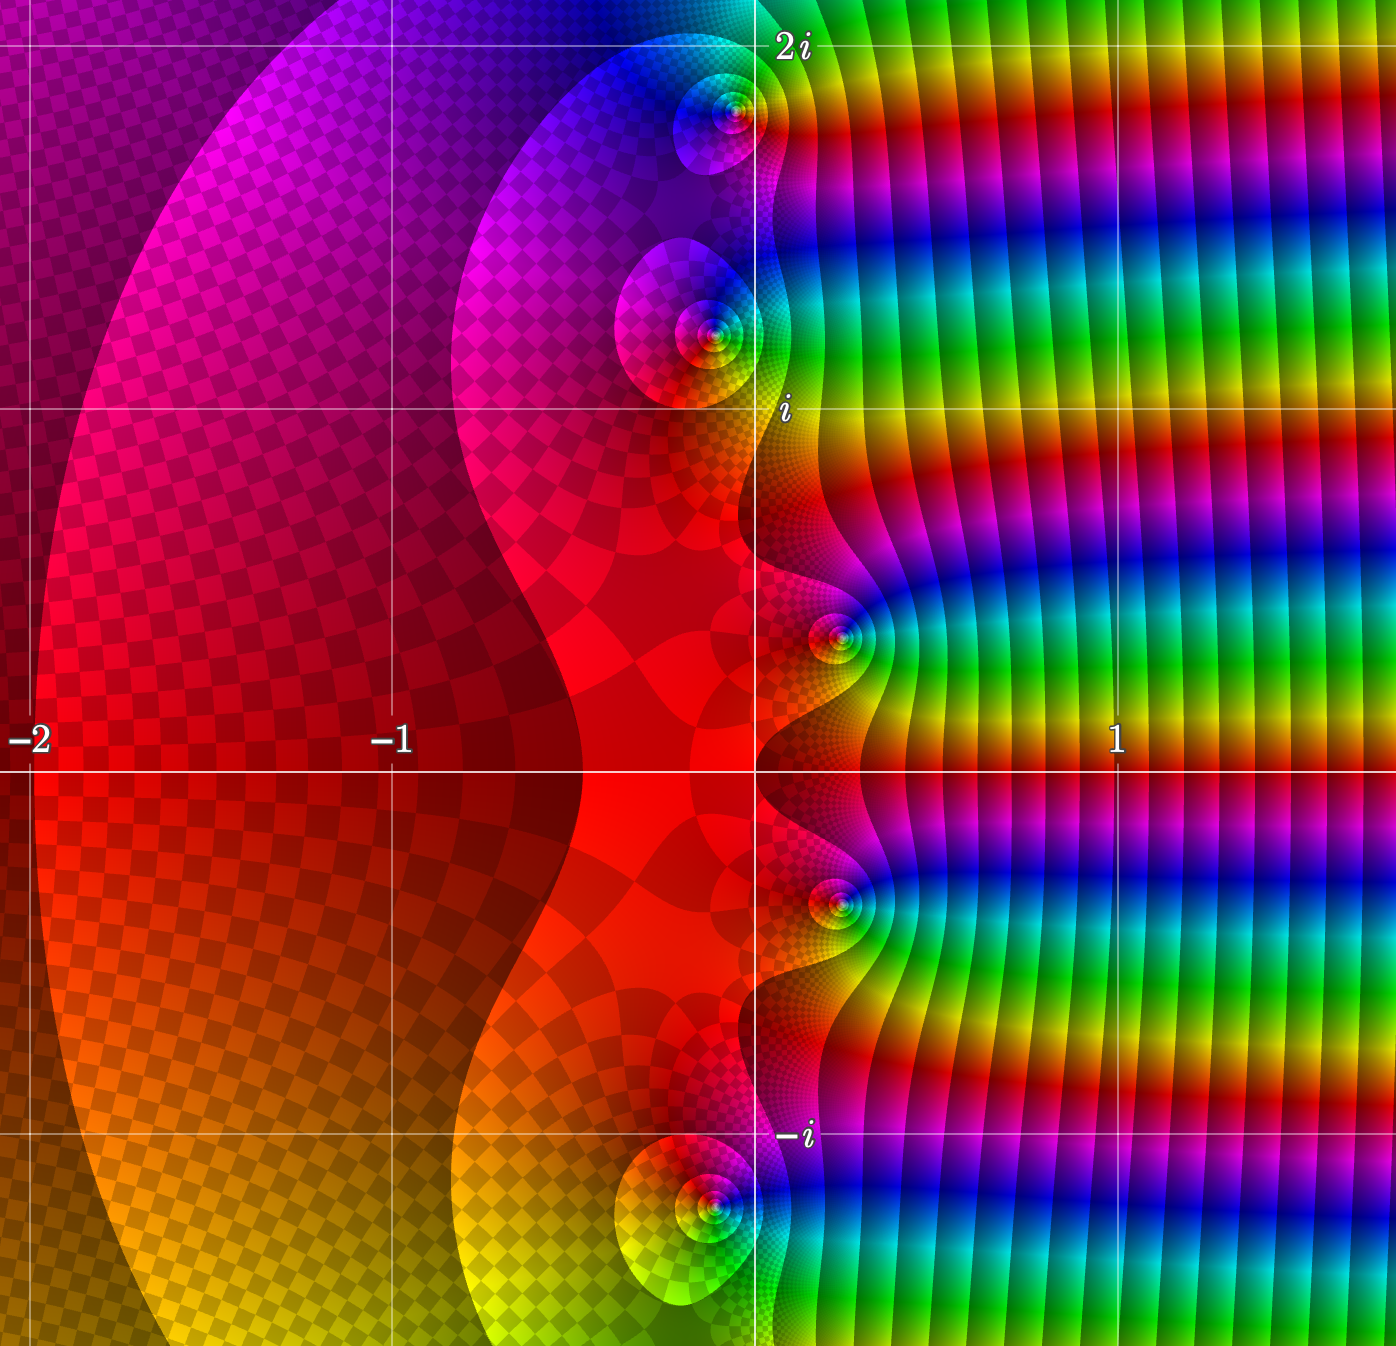
\includegraphics[width=10cm]{img/domain.png}}; 
\end{scope}

    \end{tikzpicture}
\end{center}
\newpage
    \subsection{Existence of Auxiliary Function} Assume for contradiction that as per the conditions of the theorem, $\alpha, \beta \in \A$ where $\alpha \neq 0, 1$ and $\beta \notin \Q$, but $\alpha^{\beta} \in \A$. Let $\gamma$ be a value of ${\alpha}^{\beta} = \exp(\beta \log \alpha)$. Since we are assuming for contradiction that $\alpha, \beta$, and $\gamma$ are all algebraic, we will assume there is a number field $K$ of finite degree $h$ over $\Q$ which contains $\alpha, \beta$, and $\gamma$. Using $h$, we will describe the following constants $m,q,n,t$ with the following properties:

    \begin{enumerate}
        \item{Define $m := 2h+3$.}
        \item{Find $q > 4m^2$ such that $q^2$ is a multiple of $2m$.}
        \item{Since $q^2$ is a multiple of $2m$, let their ratio be the integer $n := \frac{q^2}{2m}$}
        \item{We will also let $t := q^2 = 2mn$ since $q^2$ is ubiquitous.}
    \end{enumerate}

    These will be selected so that bounds will work out later. First, note that $q$, and as a consequence, $n$, can be selected to be arbitrarily large. We will use this later to exceed bounds. However, note that it will always be the case that $n > q$. This is because 
    \begin{align*}
        \frac{n}{q} &= \frac{\frac{q^2}{2m}}{q} & \text{(by property 3)}\\
                    &= \frac{q}{2m} \\
                    &> \frac{4m^2}{2m} &\text{(by property 2)}\\
                    &= 2m \\
                    &= 2(2h+3) &\text{(by property 1)}\\
                    &= 4h+6 \\
                    &> 1 &\text{(degree of field extension is positive)} 
    \end{align*}

    Since $\frac{n}{q} > 1$, $n > q$.\par 
    Now, consider the set $\left\{(r + k\beta)(\log \alpha) : r = 1, \ldots, q, k = 1, \ldots, q\right\}$. This set has $q^2 = t$ elements so arbitrarily name the distinct elements $\rho_1, \ldots, \rho_t$ (order of assignment does not matter). We wish to construct an auxiliary function so that we get a contradiction. Therefore, consider the entire function of the form $F: \C \to \C$ via 

\[F(z) = \sum\limits_{j=1}^{t}\eta_{j}\exp(z\rho_j)\]
where $\eta_j$'s are in $\mathcal{O}_K$. We will specify the $\eta_j$'s later to completely define this function. Now, find integer $c_1 > 0$ such that $c_1 \alpha, c_1 \beta, c_1 \gamma \in \mathcal{O}_K$. To select the $\eta_j$'s, we need the following system of equations to have a nontrivial zero: 
    \[{c_1}^{m + 2nq} {(\log \alpha)}^{-a}F^{(a)}(b) = 0\]
    for $a = 0, \ldots, n-1$ and $b = 1, \ldots, m$. Intuitively, this is so that we can get a zero of high multiplicity. Note that this system has $mn$ equations with $t = 2mn$ unknowns $\eta_j$. We want to use lemma 3.1.2, the generalized version of Siegel's lemma. Therefore, we must satisfy the hypotheses of that lemma. First, we need to bound the coefficients of the $\eta_j$'s and show they are in $\mathcal{O}_K$. Note that \[F^{(a)}(z) = \sum\limits_{i=1}^{t}(\eta_j){\rho_j}^{a}\exp(z\rho_j).\] Thus, \[F^{(a)}(b) = \sum\limits_{i=1}^{t}(\eta_j){\rho_j}^{a}\exp(b\rho_j).\] Thus, the coefficient of $\eta_j$ in the system \[{c_1}^{m + 2nq} {(\log \alpha)}^{-a}F^{(a)}(b) = 0\] is \[{c_1}^{m + 2nq} {\log(\alpha)}^{-\alpha}{\rho_j}^{a}\exp(b\rho_j)\] for each $a, b$. Substituting $\rho_j$ as $(r+k\beta)(\log \alpha)$, we get 
\begin{align*}
    {c_1}^{n+2mq}{(\log \alpha)}^{-a}\rho_j^{a}\exp(b\rho_j) &= {c_1}^{n+2mq}{(r + k\beta)}^{a}\exp\left(b(r+k\beta)(\log \alpha)\right) \\
                                                                &= {c_1}^{n+2mq}{(r+k\beta)}^{a}{\alpha}^{rb}\gamma^{kb}
\end{align*}

We therefore need to show that for all $a, b$, ${c_1}^{n+2mq}{(r+k\beta)}^{a}{\alpha}^{rb}\gamma^{kb} \in \mathcal{O}_K$. In order to do this, note that we have selected $c_1$ to make $c_1\alpha, c_1\beta, c_1\gamma \in \mathcal{O}_K$. Note that we have $a$ factors of $(r + k \beta)$, where $r, k \in \Z$ so we need $a$ factors of $c_1$ to make it in $\mathcal{O}_K$. Furthermore, we have $rb$ factors of $\alpha$ and $kb$ factors of $\gamma$. Thus, this is equivalent to determining whether the $n + 2mq$ factors of $c_1$ that we have will cover the $a + rb + kb$ terms. Note that $a, b, r, k$ are each bounded by $n-1, m, q, q$ respectively. Thus $a + rb + kb \leq n-1 + mq + q < n-1 + 2mq < n + 2mq$.\par

Now that we know ${c_1}^{n+2mq}{(r+k\beta)}^{a}{\alpha}^{rb}\gamma^{kb} \in \mathcal{O}_K$, we will find an integer upper bound on $\left\| {c_1}^{n+2mq}{(r+k\beta)}^{a}{\alpha}^{rb}\gamma^{kb} \right\|$ to apply the lemma. First, note that 

\begin{align*}
    \| r + k\beta \| &\leq \| r \| + \| k \| \| \beta \| \\
                     &\leq q + q \| \beta \| \\
                     &= q\left(1 + \| \beta \|\right)
\end{align*}

Now let $c_2 = \max\left\{\| \alpha \|, 1 + \|\beta\|, \| \gamma \|\right\}$. We will now bound the absolute values of the all conjugates of the coefficients: 
\begin{align*}
    \left\|{c_1}^{n+2mq}{(r+k\beta)}^{a}{\alpha}^{rb}\gamma^{kb}\right\| &\leq \left\| {c_1}^{n+2mq} \right\| \cdot \left\| {(r + k\beta)}^{a} \right\| \cdot \left\| {\alpha}^{rb} \right\| \cdot \left\| {\gamma}^{kb} \right\| \\
                                                              &\leq c_1^{n+2mq} \cdot {\left(q\left(1 + \| \beta \|\right)\right)}^{a} \cdot {\| \alpha \|}^{rb} \cdot {\| \gamma \|}^{kb} \\
                                                              &\leq c_1^{n+2mq} {\left({qc_2}\right)}^{a} \left({c_2}^{rb}\right) \left({c_2}^{kb}\right) \\
                                                              &\leq c_1^{n+2mq} {\left({qc_2}\right)}^{n} \left({c_2}^{2mq}\right) \\
                                                              &= {\left(c_{1}c_{2}\right)}^{n} {\left(c_{1}c_{2}\right)}^{2mq}q^{n} \\
                                                              &=  {\left(c_{1}c_{2}\right)}^{n} {\left(c_{1}c_{2}\right)}^{2mq}{\left(\sqrt{2mn}\right)}^{n} \\
                                                              &= {\left(c_{1}c_{2}\right)}^{n} {\left(c_{1}c_{2}\right)}^{2mq}{\left(\sqrt{2m}\right)}^{n}n^{\frac{n}{2}}
\end{align*}

Now, we will further bound this using the constant $c_3 := {\left(c_{1}c_{2}\right)}^{2m+1}\sqrt{2m}$. Therefore, recalling that $n > q$, 

\begin{align*}
    {\left(c_{1}c_{2}\right)}^{n} {\left(c_{1}c_{2}\right)}^{2mq}{\left(\sqrt{2m}\right)}^{n}n^{\frac{n}{2}} &< {(c_{1}c_{2})}^{n}{(c_{1}c_{2})}^{2mn}{\left(\sqrt{2m}\right)}^{n}n^{\frac{n}{2}} \\
                                                                                                             &= {\left({(c_{1}c_{2})}^{2m+1}\right)}^{n}{\left(\sqrt{2m}\right)}^{n}n^{\frac{n}{2}} \\
                                                                                                             &= {\left({(c_{1}c_{2})}^{2m+1}\sqrt{2m}\right)}^{n}{n}^{\frac{n}{2}} \\
                                                                                                             &= {c_3}^{n}n^{\frac{n}{2}}
\end{align*}

Now, we are ready to apply the lemma. We get that we can find nontrivial $\| \eta_j \|$ such that for every $j$, 

\begin{align*}
    \| \eta_j \| &< c + c{\left(c\left(2mn\right){c_3}^{n}n^{\frac{n}{2}}\right)}^{\frac{mn}{2mn - mn}} \\
                 &= c + 2c^{2}mn{c_{3}}^{n}n^{\frac{n}{2}} \\
                 &< 3{c}^{2}mn{c_{3}}^{n}{n}^{\frac{n}{2}} 
\end{align*}
}

From the lemma, $c$ is dependent only on $K$ and is independent of $n$. Also, note this is also the case with $c_3$ because it was defined independently of $n$ and only in terms of other constants related to $\alpha, \beta$ and $\gamma$. Note that $2^{n} > n > q > m$ so $4^{n} > mn$. Thus, continuing the inequality, we get,

\begin{align*}
    3{c}^{2}mn{c_{3}}^{n}{n}^{\frac{n}{2}} &< 3{c}^{2}{(4c_3)}^{n}n^{\frac{n}{2}} \\ 
                                           &< {c_4}^{n}n^{\frac{n}{2}}
\end{align*}

where $c_4 := \left(4{c}^{2}\right)\left(4c_3\right)$. Note  that $c_4$ is still independent of $n$. We will use this as the final bound for $\| \eta_j \|$. We therefore know that there exists an auxiliary function $F$ with a nontrivial zero of high multiplicity such that it solves the system of equations 
\[{c_1}^{m + 2nq} {(\log \alpha)}^{-a}F^{(a)}(b) = 0\]
for all $a,b$ with $\| \eta_j \| < {c_4}^{n}n^{\frac{n}{2}}$ for all algebraic integers $\eta_j$ in the system.

\subsection{Analysis of Auxiliary Function}
First, we will show that the function's derivatives will not always vanish from $1$ to $m$ past a certain number of derivatives. More specifically, there are $p, B \in \Z$ where $p \geq n$ and $1 \leq B \leq m$ such that $F^{(a)}(b) = 0$ for $a = 1, \ldots, p-1$ and $b = 1, \ldots, m$ but $F^{(p)}(B) \neq 0$.\par

To see this, suppose for contradiction that for all $a = 0, \ldots, t-1$, the derivative vanishes. Note that \[F^{(a)}(B) = \sum\limits_{j=1}^{t} \eta_{j}{\rho_{j}}^{a}\exp(B\rho_j).\] We therefore get the system of $a$ equations \[F^{(a)}(B) = \sum\limits_{j = 1}^{t} \eta_{j}{\left(\rho_j\right)}^{a}\exp(B\rho_j) = 0.\]

In matrix form, we can write this system as 

\[
    \begin{pmatrix}
        1 & 1 & \hdots & 1 \\
        \rho_{1} & \rho_{2} & \hdots & {\rho_t} \\ 
        \vdots & \vdots & \ddots & \vdots \\
        {\rho_{1}}^{t-1} & {\rho_{2}}^{t-1} & \hdots & {\rho_t}^{t-1}
    \end{pmatrix} 
    \begin{pmatrix}
        \exp(B\rho_1) & 0 & \hdots & 0 \\
        0 & \exp(B\rho_2) & \hdots & 0 \\
        \vdots & \vdots & \ddots & \vdots \\
        0 & 0 & \hdots & \exp(B\rho_t) 
    \end{pmatrix} 
    \begin{pmatrix}
        \eta_1 \\ \eta_2 \\ \vdots \\ \eta_t
    \end{pmatrix} = 
    \begin{pmatrix}
        0 \\ 0 \\ \vdots \\ 0
    \end{pmatrix} 
\]

Note that since our auxiliary function was constructed so that the $\eta_j$'s were not all zero (nontrivial solution), it must be the case that 

\[
    \begin{pmatrix}
        1 & 1 & \hdots & 1 \\
        \rho_{1} & \rho_{2} & \hdots & {\rho_t} \\ 
        \vdots & \vdots & \ddots & \vdots \\
        {\rho_{1}}^{t-1} & {\rho_{2}}^{t-1} & \hdots & {\rho_t}^{t-1}
    \end{pmatrix} 
    \begin{pmatrix}
        \exp(B\rho_1) & 0 & \hdots & 0 \\
        0 & \exp(B\rho_2) & \hdots & 0 \\
        \vdots & \vdots & \ddots & \vdots \\
        0 & 0 & \hdots & \exp(B\rho_t) 
    \end{pmatrix}\] 

is not full rank. Therefore, its determinant is $0$. Note that the determinant of the diagonal matrix

\[\begin{pmatrix}
        \exp(B\rho_1) & 0 & \hdots & 0 \\
        0 & \exp(B\rho_2) & \hdots & 0 \\
        \vdots & \vdots & \ddots & \vdots \\
        0 & 0 & \hdots & \exp(B\rho_t) 
    \end{pmatrix}\]
is the product of the entries along its diagonal: $\prod\limits_{j=1}^{t}\exp(B\rho_{j})$, which cannot be zero. Therefore, it must be the case that the determinant of 

\[\begin{pmatrix}
        1 & 1 & \hdots & 1 \\
        \rho_{1} & \rho_{2} & \hdots & {\rho_t} \\ 
        \vdots & \vdots & \ddots & \vdots \\
        {\rho_{1}}^{t-1} & {\rho_{2}}^{t-1} & \hdots & {\rho_t}^{t-1}
    \end{pmatrix}\] 

    is zero. Note that this is the transpose of the Vandermonde matrix $V(\rho_1, \ldots, \rho_t)$. Therefore, it must be the case that there is $\rho_i = \rho_j$ where $i \neq j$. This would mean there is $\left(r_1 + k_1 \beta \right)\log \alpha = \left(r_2 + k_2 \beta\right) \log \alpha$ for $r_1, r_2, k_1, k_2 \in \{1, \ldots, q\}$. Note that since $\alpha \neq 0, 1$ it must be the case that $\log \alpha \neq 0$. Thus, we can say that $r_1 + k_1 \beta = r_2 + k_2 \beta$. It cannot be the case that $k_1 = k_2$ since that would force $r_1 = r_2$ and the two terms would be equal. Therefore, $k_2 - k_1 \neq 0$. From this, we can deduce that  
    \begin{align*}
        r_1 + k_1 \beta = r_2 + k_2 \beta &\implies r_1 - r_2 = (k_2 - k_1) \beta \\
                                          &\implies \frac{r_1 - r_2}{k_2 - k_1} = \beta
    \end{align*}
for integers $r_1, r_2, k_1, k_2$, which would be a contradiction since that would imply $\beta \in \Q$.\par

From this we confirmed that the auxiliary function vanishes at $B$ for the first $n$ derivatives, but there is $p$ such that $F^{(p)}(B) \neq 0$. Let 

\begin{align*}
    \zeta &:= {(\log \alpha)}^{(-p)}F^{(p)}(B) \\
          &= \sum\limits_{j=1}^{t}\eta_{j}{\left(\log(\alpha)\right)}^{-p}{\rho_{j}}^{p}\exp(B\rho_j) \\
          &= \sum\limits_{j=1}^{t} \eta_{j}{\left(r_j + k_j \beta\right)}^{p}{\alpha}^{Br_{j}}{\gamma}^{Bk_{j}} \\
\end{align*}
where $r_j, k_j$ are in $\{1, \ldots, q\}$. Note that $\zeta \neq 0$ because we showed $F^{(p)}(B) \neq 0$.\par

Next, there is $C > 0$ independent of $n$ and $p$ such that 

\[\vert N_{K}(\zeta) \vert \geq C^{-p}.\]

To see this, recall that $c_1$ is the positive integer constant which makes $c_1\alpha, c_1\beta, c_1\gamma \in \mathcal{O}_K$. Using a similar argument from before, ${c_1}^{p+2mq} \zeta = {c_1}^{p + 2mq}\sum\limits_{j=1}^{t}{\eta_{j}\left(r_j + k_j \beta\right)}^{p}{\alpha}^{Br_{j}}{\gamma}^{Bk_{j}} \in \mathcal{O}_K$ as $m$ upper bounds $B$ and $q$ upper bounds $r_j$ and $k_j$. This helps us verify that we have enough factors of $c_1$ to make $\zeta$ an algebraic integer. We can let $c_5 := {c_1}^{2m+1}$ so ${c_5}^p = {c_1}^{2mp + p}$ upper bounds ${c_1}^{p + 2mq}$ from the fact that $q < n \leq p$. Thus, ${c_5}^{p}\zeta \in \mathcal{O}_K$ so its norm in $K$ is an integer. Furthermore, its norm is nonzero because $\zeta$ is nonzero.  We can conclude from this that $\vert N_K({c_5}^{p}\zeta) \vert \geq 1$. Thus,

\begin{align*}
    1 &\leq \vert N_K({c_5}^{p}\zeta) \vert \\
      &= \vert N_K({c_5}^{p}) N_K(\zeta) \vert \\
      &\leq \vert N_K({c_5}^{p}) \vert \cdot \vert N_K(\zeta) \vert \\
      & \leq C^{p}\vert N_K(\zeta) \vert
\end{align*}

Thus, we get that $\vert N_K(\zeta) \vert \geq C^{-p}$ for some constant $C = {c_5}^{h}$ independent of $n$ and $p$.\par

Next, we will establish that there is another constant $c$, independent of $n$ and $p$ such that \[\| \zeta \| < c^{p}p^{p}.\]

To get this bound, note that 
\begin{align*}
    \| \zeta \| &= \left\| \sum\limits_{j=1}^{t} \eta_{j}{\left(r_j + k_j \beta\right)}^{p}{\alpha}^{Br_{j}}{\gamma}^{Bk_{j}} \right\| \\
                &\leq \sum\limits_{j=1}^{t} \left\| \eta_{j}{\left(r_j + k_j \beta\right)}^{p}{\alpha}^{Br_{j}}{\gamma}^{Bk_{j}} \right\| \\
                &\leq \sum\limits_{j=1}^{t} \left\| \eta_{j} \right\| \cdot {\left\| r_j + k_j \beta \right\|}^{p} \cdot  {\left\| \alpha \right\|}^{Br_{j}}  \cdot  {\left\| \gamma \right\|}^{Bk_{j}}  \\
                &\leq t \cdot \max_{j} \left\{ \left\| \eta_{j} \right\| \cdot {\left\| r_j + k_j \beta \right\|}^{p} \cdot  {\left\| \alpha \right\|}^{Br_{j}}  \cdot  {\left\| \gamma \right\|}^{Bk_{j}} \right\}
\end{align*}

To further bound this, first note that $q < n \leq p$. Then, $t = 2mn < 2^{n}$ for sufficiently large $n$. Now, $r, k, b, \| \alpha \|, 1 + \| \beta \|, \gamma$ can be upper bounded by $q,q,m,c_2, c_2, c_2$ respectively. Also, recall that $\| \eta_j \| < {c_4}^{n}n^{\frac{n}{2}}$ so
\begin{align*}
    t \cdot \max_{j} \left\{ \left\| \eta_{j} \right\| \cdot {\left\| r_j + k_j \beta \right\|}^{p} \cdot  {\left\| \alpha \right\|}^{Br_{j}}  \cdot  {\left\| \gamma \right\|}^{Bk_{j}} \right\} &< 2^{n}\left({c_4}^{n}n^{\frac{n}{2}}\right){\left(qc_2\right)}^{p}\left({{c_{2}}}^{mq}\right)\left({{c_{2}}}^{mq}\right) \\
                                                                                                                                                                                                  &\leq {\left(2c_{4}{c_{2}}^{1+2m}\right)}^{p}{n}^{\frac{n}{2}}{q}^{p}
\end{align*}

Note that
\begin{align*}
    q^p &= {\left(\sqrt{2mn}\right)}^{p} \\ 
        &= {\left(\sqrt{2m}\right)}^{p}{n}^{\frac{p}{2}} \\
        &\leq {\left(\sqrt{2m}\right)}^{p}{p}^{\frac{p}{2}}
\end{align*}
and as a result of $n \leq p$, \[n^{\frac{n}{2}} \leq p^{\frac{p}{2}}.\]

Putting this all together, we get that
\begin{align*}
    \| \zeta \| &< {\left(2c_{4}{c_{2}}^{1+2m}\right)}^{p}{n}^{\frac{n}{2}}{q}^{p} \\
                &\leq {\left(2c_{4}{c_{2}}^{1+2m}\right)}^{p}\left({p}^{\frac{p}{2}}\right){\left(\sqrt{2m}\right)}^{p}\left({p}^{\frac{p}{2}}\right) \\
                &= {\left(2c_{4}{c_{2}}^{1+2m}\sqrt{2m}\right)}^{p}{p}^{p} \\
                &= {c}^{p}{p}^{p}
\end{align*}
For $c := 2c_{4}{c_{2}}^{1+2m}\sqrt{2m}$, which is a constant independent of $n$ and $p$.\par

We will now define another function $S : \C \to \C$ via (the analytic continuation of)
\[S(z) = p! F(z) \left(\prod\limits_{b=1}^{m} {(z - b)}^{-p}\right)\left(\prod\limits_{\substack {b = 1 \\ b \neq B}}^{m} {(B - b)}^{p}\right).\]

Note that $S$ is also entire because the function $F(z)$ is entire and the multiplicity of the zeroes at $z = 1, \ldots, m$ is at least $p$. We are using the analytic continuation of the function written above so that it can still be defined at $z = B$ even though there is a ${(B-B)}^{p}$ in the denominator. By the Taylor series expansion of $F$ at $B$, we get that 
\[F(z) = \sum\limits_{k = p}^{\infty} \frac{{(z-B)}^{k}F^{(k)}(B)}{k!}.\]

Therefore, substituting, we get that

\[S(z) = p! \left(\sum\limits_{k = p}^{\infty} \frac{{(z-B)}^{k}F^{(k)}(B)}{k!}\right) \left(\prod\limits_{b=1}^{m} {(z - b)}^{-p}\right)\left(\prod\limits_{\substack {b = 1 \\ b \neq B}}^{m} {(B - b)}^{p}\right).\]

Therefore, \[S(B) = F^{(p)}(B)\] as the ${(B-B)}^{p}$ term is only in the denominator when $k = p$. Furthermore, this gives us that \[\zeta = {(\log \alpha)}^{-p}F^{(p)}(B) = {(\log \alpha)}^{-p}S(B).\]

Take a simple closed curved around $z = B$, specifically, the circle $\mathcal{C} := \left\{z : \vert z \vert = \frac{p}{q}\right\}$. Note that this circle contains $B$ because \[\frac{p}{q} > \frac{p}{2q} \geq \frac{n}{2q} = \frac{q}{4m} > m \geq B.\] By Cauchy's Residue theorem, we get that \[S(B) = \frac{1}{2 \pi i}\oint_{\mathcal{C}} \frac{S(z)}{z-B} dz.\]

Recall that $\vert \eta_j \vert < {c_4}^{n}{n}^{\frac{n}{2}}$ and note that for all $z$, $\vert \exp(z\rho_j) \vert \leq  \exp(\vert z\rho_j \vert)$. Our goal is to eventually find a bound on $\vert F(z) \vert$. First, we will complete bounding $\vert \exp(z\rho_j) \vert$:

\begin{align*}
    \vert \exp(z\rho_j) \vert &\leq \exp(\vert z\rho_j \vert) \\
                              &= \exp\left(\vert z \vert \cdot \vert \rho_j \vert\right) \\
                              &\leq \exp\left(\frac{p}{q}\left(q + q \vert \beta \vert\right) \log \alpha\right) \\
                              &= \exp(p(1 + \vert \beta \vert) \log \alpha) \\
                              &= {c_6}^{p}
\end{align*}
for $c_6 := \exp((1 + \vert \beta \vert) \log \alpha)$. Now, we will bound $\vert F(z) \vert$.
\begin{align*}
    \vert F(z) \vert &= \left\vert \sum\limits_{j=1}^{t} \eta_{j}\exp(z\rho_j)\right\vert \\
                     &\leq t \cdot \max_{j} \left\vert \eta_j \exp(z\rho_j) \right\vert \\
                     &= t \cdot \max_{j} \left\vert \eta_j \right\vert \cdot \left\vert \exp(z\rho_j) \right\vert \\
                     &< t{c_4}^{n}{n}^{\frac{n}{2}}{c_6}^{p} \\
                     &< 2^{n}{c_4}^{n}{c_6}^{p}{n}^{\frac{n}{2}} \\
                     &\leq 2^{p}{c_4}^{p}{c_6}^{p}{n}^{\frac{n}{2}} \\
                     &= {\left(2c_{4}c_{6}\right)}^{p}{n}^{\frac{n}{2}} \\
                     &={c_7}^{p}{p}^{\frac{p}{2}} 
\end{align*}

for $c_7 := 2c_{4}c_{6}$.\par

Next, we will bound ${\vert z - b \vert}^{-p}$. Recall that \[\frac{p}{2q} > m.\] Then,
\begin{align*}
    \vert z - b \vert &\geq \vert z \vert - \vert b \vert \\
                      &\geq \frac{p}{q} - m \\
                      &\geq \frac{p}{2q}
\end{align*}
Therefore, \[{\vert z - b \vert}^{-p} \leq {\left(\frac{2q}{p}\right)}^{p}.\] Now, we can bound $\vert S(z) \vert$.
\begin{align*}
    \vert S(z) \vert &= \left\vert p! F(z) \left(\prod\limits_{b=1}^{m} {(z - b)}^{-p}\right)\left(\prod\limits_{\substack {b = 1 \\ b \neq B}}^{m} {(B - b)}^{p}\right) \right\vert \\
                     &\leq \left\vert p!\right\vert \cdot \left\vert F(z)\right\vert \cdot \left\vert \left(\prod\limits_{b=1}^{m} {(z - b)}^{-p}\right)\right\vert \cdot \left\vert \left(\prod\limits_{\substack {b = 1 \\ b \neq B}}^{m} {(B - b)}^{p}\right) \right\vert \\
                     &< (p!)\left({c_7}^{p}{p}^{\frac{p}{2}}\right){\left(\frac{2q}{p}\right)}^{mp}\left(\prod\limits_{\substack {b = 1 \\ b \neq B}}^{m} {(B - b)}^{p}\right) \\
                     &= (p!)\left({c_7}^{p}{p}^{\frac{p}{2}}\right){\left(\frac{2\sqrt{2mn}}{p}\right)}^{mp}\left(\prod\limits_{\substack {b = 1 \\ b \neq B}}^{m} {(B - b)}^{p}\right) \\
                     &= {\left(c_{7}2^{m}{(2m)}^{\frac{m}{2}} \prod\limits_{\substack {b = 1 \\ b \neq B}}^{m} {(B - b)}^{p}\right)}^{p}(p!)\left(p^{\frac{p}{2}}\right){\left(\frac{\sqrt{n}}{p}\right)}^{mp} \\
                     &= {c_8}^{p}(p!)p^{\frac{p}{2}}{\left(\frac{\sqrt{n}}{p}\right)}^{mp} 
\end{align*}
for \[c_8 := \left(c_{7}2^{m}{(2m)}^{\frac{m}{2}} \prod\limits_{\substack {b = 1 \\ b \neq B}}^{m} {(B - b)}^{p}\right).\] To further bound this, note that $p! < p^{p}$ and as $n \leq p$, \[\frac{\sqrt{n}}{p} = \frac{\frac{\sqrt{n}}{\sqrt{p}}}{\sqrt{p}} \leq \frac{1}{\sqrt{p}}.\]

Therefore, for $z$ on $\mathcal{C}$,
\begin{align*}
    {c_8}^{p}(p!)p^{\frac{p}{2}}{\left(\frac{\sqrt{n}}{p}\right)}^{mp} &\leq {c_8}^{p}(p^{p})p^{\frac{p}{2}}{\left(\frac{1}{p}\right)}^{mp} \\
                                                                       &= {c_8}^{p}p^{\frac{p(3-m)}{2}}
\end{align*}

Now, we will bound $\vert \zeta \vert$.
\begin{align*}
    \vert \zeta \vert &= \left\vert {(\log \alpha)}^{-p} S(B) \right\vert \\
                      &\leq {\vert \log \alpha \vert}^{-p} \cdot \vert S(B) \vert \\
                      &= {\vert \log \alpha \vert}^{-p} \cdot \left\vert \frac{1}{2 \pi i} \oint_{\mathcal{C}} \frac{S(z)}{z-B} dz \right\vert \\
                      &= \frac{1}{2\pi} \cdot {\vert \log \alpha \vert}^{-p} \cdot \left\vert\oint_{\mathcal{C}} \frac{S(z)}{z-B} dz \right\vert 
\end{align*}

To compute a bound on \[\left\vert \oint_{\mathcal{C}} \frac{S(z)}{z-B} dz\right\vert,\] note that the path of integration along $\mathcal{C}$ has length $\frac{2 \pi p}{q}$ and since $\vert S(z) \vert \leq {c_8}^{p}p^{\frac{p(3-m)}{2}}$, and $\vert z - b \vert \geq \frac{p}{2q}$, the maximum of $\left\vert \frac{S(z)}{z-B} \right\vert$ is bounded by $\frac{{c_8}^{p}p^{\frac{p(3-m)}{2}}}{\frac{p}{2q}}$. By the maximum modulus principle, we get that \[\left\vert \oint_{\mathcal{C}} \frac{S(z)}{z-B} dz\right\vert \leq \frac{2 \pi p}{q} \left(\frac{{c_8}^{p}p^{\frac{p(3-m)}{2}}}{\frac{p}{2q}}\right)\]

Therefore, 
\begin{align*}
    \vert \zeta \vert &< \frac{1}{2\pi} \cdot {\vert \log \alpha \vert}^{-p} \cdot \frac{2 \pi p}{q} \left(\frac{{c_8}^{p}p^{\frac{p(3-m)}{2}}}{\frac{p}{2q}}\right)\\
                      &= {\vert \log \alpha \vert}^{-p} \cdot \frac{p}{q} \cdot {c_8}^{p}p^{\frac{p(3-m)}{2}} \cdot \frac{2q}{p} \\
                      &< {\left(2c_8 {\vert \log \alpha \vert}^{-1}\right)}^{p}p^{\frac{p(3-m)}{2}} \\
                      &= {c_9}^{p}{p}^{\frac{p(3-m)}{2}} 
\end{align*}

For $c_9 := 2c_8 {\vert \log \alpha \vert}^{-1}$. Recall that $\| \zeta \| < c^{p}p^{p}$. We know $\vert \zeta \vert < {c_9}^{p}{p}^{\frac{p(3-m)}{2}}$ so we know that $\vert N_K(\zeta) \vert$ cannot exceed $\vert \zeta \vert \cdot {\| \zeta \|}^{h-1}$ as we know at least one of the $h$ embeddings goes to $\zeta$ and the remaining $h-1$ cannot have absolute value exceeding $\| \zeta \|$. Therefore, 

\begin{align*}
    \vert N_K(\zeta) \vert &\leq \vert \zeta \vert \cdot {\| \zeta \|}^{h-1} \\
                           &< \left({c_9}^{p}{p}^{\frac{p(3-m)}{2}}\right){\left(c^{p}p^{p}\right)}^{h-1} \\
                           &= {(c_{9}c^{h-1})}^{p}p^{-p} \\
                           &= {c_{10}^{p}p^{-p}}
\end{align*}

for $c_{10} := c_{9}c^{h-1}$. Note that $c_{10}$ is also independent of $n$ and $p$. However, recall that $\vert N_K(\zeta) \vert \geq C^{-p}$. Therefore,

\[{c_{10}^{p}p^{-p}} > \vert N_K(\zeta) \vert \geq C^{-p}\]

so \[{c_{10}}^{p}p^{-p} > C^{-p}.\] Rearranging terms and canceling out the powers, we get \[Cc_{10} > p,\] where $C, c_{10}$ are independent of $n, p$ and only depend on $K$. However, since $n \leq p$, we can choose $n$ and therefore $p$ arbitrarily large, which is a contradiction.\par

This proves the Gelfond-Schneider theorem because it implies that it cannot be the case that all $\alpha, \beta, \gamma \in \A$. By the hypothesis $\alpha, \beta \in \A$ so it must be the case that $\gamma$, any value of $\alpha^{\beta}$ is transcendental.\par

\[\greenlozenge\]

\newpage
\section{Consequences}

\begin{mybox}
    \theorem{The Gelfond-Schneider constant $2^{\sqrt{2}}$, Gelfond's constant $e^{\pi}$, and $e^{-\frac{\pi}{2}}$ are transcendental.}
\end{mybox}

\proof{Showing $2^{\sqrt{2}}$ is transcendental is a direct application of the main theorem and is shown by verifying that $2$ is algebraic, not $0$ nor $1$, and also that $\sqrt{2} \notin \Q$.\par

Note, we cannot use the direct application of the Gelfond-Schneider theorem for $e^{\pi}$ because we have shown that $e$ is transcendental by the Lindemann-Weierstrass theorem. However, using Euler's identity, we can rewrite (noting that $\frac{1}{i} = -i$) it via \[e^{\pi} = {\left(e^{\pi i}\right)}^{\frac{1}{i}} = {\left(e^{\pi i}\right)}^{-i} = {(-1)}^{-i}.\] Since $-1$ is neither $0$ nor $1$ and is algebraic, $i$ is algebraic but not in $\Q$, we know $e^{\pi}$ must be transcendental. Since we cannot do the same trick for $\pi^{e}$, the transcendence of $\pi^{e}$ is still unknown.\par 

For $e^{-\frac{\pi}{2}}$, we can use Euler's identity as before to get ${\left(e^{-\frac{\pi i}{2}}\right)}^{i} = i^i$. Therefore, this is also transcendental. We can also use the fact that $e^{\pi}$ is transcendental and the function $x \mapsto x^{-\frac{1}{2}}$ is an algebraic function. Therefore, $e^{-\frac{\pi}{2}}$ must be transcendental.\par
\[\greenlozenge\]}

\newpage
\begin{mybox}
    \theorem{Let $a, b \in \Z$ be positive such that they are not powers of the same positive integer and $a \neq 1$. Then $\log_{b}(a)$ is transcendental.}
\end{mybox}
\proof{Let $c = \log_b(a)$. Then, ${b}^{c} = a$. Note that since $a \neq 1$ and is positive, $b$ is neither $0$ nor $1$. Then, we know that since $a \in \Z$, it cannot be transcendental. Thus, the hypothesis of the Gelfond-Schneider theorem fails. We know that $b$ is an integer not in $\{0, 1\}$ so it must be the case that either $c \in \Q$ or $c \notin \A$. Suppose for contradiction that $c \in \Q$ so $c = \frac{p}{q}$ for integers $p, q$ and $q$ is nonzero. Then, since $\log_{b}(a) = \frac{p}{q}$, we know $b^{\frac{p}{q}} = a$ so $b^{p} = a^{q}$. From this, we can tell that $p$ must also be nonzero since $a \neq 1$ and $q \neq 0$. However, since $a$ and $b$ are not powers of the same positive integer, there is prime $r$ such that $r \mid a$, but $r \nmid b$. Thus, $\nu_{r}(a^{p}) > 0$, but $\nu_{r}(b^{q}) = 0$, which is a contradiction. This means $c = \log_{b}(a)$ must be transcendental.\par \[ \greenlozenge \]}
\chapter{Baker's Theorem}
\section{Baker 1966}
\begin{mybox}
    \theorem{(Baker's 1966 Theorem) Let nonzero $\alpha_1, \ldots, \alpha_n \in \A$. Then, if $2\pi i, \log(\alpha_1), \ldots, \log(\alpha_{n})$ are $\Q$-linearly independent, they are also $\A$-linearly independent.}
\end{mybox}
\note{This proof uses the auxiliary function

\[F(z_1, \ldots, z_n) = \] \[\sum\limits_{\lambda_1 = 0}^{L}\sum\limits_{\lambda_2=0}^{L} \cdots \sum\limits_{\lambda_n = 0}^{L}p(\lambda_1, \lambda_2, \ldots, \lambda_n)\alpha_1^{(\lambda_1 + \lambda_n\beta)z_1}\cdots \alpha_{n-1}^{(\lambda_{n-1}+\lambda_{n}\beta)z_{n-1}}\]

in a very similar way to the Gelfond-Schneider theorem. In particular, it uses Siegel's lemma to show the existence of this function.}

\newpage
\section{Baker 1967a}
\begin{mybox}
    \theorem{(Baker's 1967a Theorem) Let nonzero $\alpha_1, \ldots, \alpha_n \in \A$. Then, if $\log(\alpha_1), \ldots, \log(\alpha_{n})$ are $\Q$-linearly independent, they are also $\A$-linearly independent.}
\end{mybox}
\note{Baker later showed how to remove the $2\pi i$ from the previous proof by changing the conditions at the conclusion.}

\newpage
\section{Baker 1967b}
\begin{mybox}
    \theorem{(Baker's 1967b Theorem)  Let nonzero $\alpha_1, \ldots, \alpha_n \in \A$. Then if $\log(\alpha_1), \ldots, \log(\alpha_{n})$ are $\Q$-linearly independent, and $\beta_0, \beta_1, \ldots, \beta_n$ are nonzero algebraic numbers, then 
    \[\left\vert \beta_0 + \beta_1\log(\alpha_1) + \cdots + \beta_n\log(\alpha_n) \right\vert > H^{-C}\] where $H$ is the maximum of the heights of the $\beta_i$'s and $C$ is effectively computable depending on $n$, $\lambda_i$'s, and the maximum degrees of $\beta$.}
\end{mybox}
\note{This was the inequality that resulted from analyzing the auxiliary function in Baker 1966.}

\newpage
\section{Consequences}
Baker's theorem generalizes the Lindemann-Weierstrass and Gelfond-Schneider theorems. For $a_1, \ldots, a_n \in \A$ not $0$ or $1$, and $\beta_1, \ldots, \beta_n \in \A \setminus \Q$ and $\Q$-linearly independent, ${a_1}^{\beta_1}\cdots {a_n}^{\beta_n}$ is transcendental.\par
\chapter{Schanuel's Conjecture}
\begin{mybox}
    \conjecture{(Schanuel's Conjecture) Suppose we have $n$ complex numbers \[z_1, \ldots, z_n\] that are linearly independent over $\Q$. Then, $\Q(z_1, \ldots, z_n, e^{z_1}, \ldots, e^{z_n})$ has transcendence degree at least $n$ over $\Q$.}
\end{mybox}
\newpage
\section{Consequences}
This proves most questions in transcendental number theory. Setting $z_1 = 1, z_2 = \pi i$ shows algebraic independence of $e$ and $\pi$. Setting $z_1 = 1$, $z_2 = e$ shows transcendence of $e^{e}$.
        Setting $z_1 = \log \log \pi, z_2 = 1 + \log \log \pi, z_3 = \log \pi, z_4 = e \log \pi, z_5 = i \pi$, one can show $\pi^{e}$ is transcendental. 
\newpage
\section{Converse Conjecture}
\begin{mybox}
    \theorem{(Converse Schanuel conjecture) If $F$ is a countable field with charactersitic $0$, $e: F \to F$ is a field homomorphism from the additive group to the multiplicative group whose kernel is cyclic, and \[\trdeg(\Q(x_1, \ldots, x_n, e(x_1), \ldots, e(x_n))/\Q) \geq n,\]then there is a field homomorphism $h : F \to \C$ such that $h(e(x)) = \exp(h(x))$ for all $x \in F$.}
\end{mybox}

\note{This is denoted as the converse and is also an open problem.}

\newpage
\section{Progress}
In 1971, James Ax proved a similar statement of the conjecture for formal power series. That is, for any $n$ formal power series $f_1, \ldots, f_n \in t\C[[t]]$ which are $\Q$-linearly independent, the field extension $\C(t, f_1, \ldots, f_n, \exp(f_1), \ldots, \exp(f_n))$ has transcendence degree at least $n$ over $\C(t)$.\par

In 2004, Boris Zilber constructed an exponential field using methods from model theory with Schanuel's conjecture as an axiom. If it can be shown that that is isomorphic to $\C$, that would imply Schanuel's conjecture.

\backmatter{}
\printindex
\newpage{}
\begin{thebibliography}{99} % Beamer does not support BibTeX so references must be inserted manually as below, you may need to use multiple columns and/or reduce the font size further if you have many references
		\footnotesize % Reduce the font size in the bibliography
	
		\bibitem[Niven, 1956]{p1}
			 Ivan Niven
             \newblock{Irrational Numbers}

        \bibitem[Conway, 1996]{p2}
            John Conway
            \newblock{The Look and Say Sequence}

		\bibitem[Burger, 2004]{p3}
            Edward Burger 
            \newblock{Making Transcendence Transparent}

            \bibitem[Wolfram MathWorld]{p4}
            Wolfram MathWorld
            \newblock{Schanuel's Conjecture}
        
            \bibitem[Gelfond, 1959]{p5}
            Alexander Gelfond
            \newblock{Transcendental and Algebraic Numbers}

        \bibitem[Baker, 1975]{p6}
            Alan Baker 
            \newblock{Transcendental Number Theory}

        \bibitem[Soundararajan, 2011]{p7}
            Kannan Soundararajan
            \newblock{Transcendental Number Theory}

	\end{thebibliography} 
\end{document}
